%%-*-latex-*-

\documentclass[wide]{slides}

% Language
%
\usepackage{hyphenat}          % \hyp{} is a breakable dash
\usepackage{alltt}
\usepackage{xspace}

\frenchspacing  % Follow French conventions after a period

% Graphics
%
\usepackage{graphicx}

% Maths & Logic
%
\usepackage{amsmath,amssymb,amsthm,stmaryrd}
\usepackage{mathpartir}

% New commands
%
% PascaLIGO

\newcommand{\Kand}[0]{\textbf{and}\xspace}
\newcommand{\Kattributes}[0]{\textbf{attributes}\xspace}
\newcommand{\Kbegin}[0]{\textbf{begin}\xspace}
\newcommand{\Kbigmap}[0]{\textbf{big_map}\xspace}
\newcommand{\Kblock}[0]{\textbf{block}\xspace}
\newcommand{\Kcase}[0]{\textbf{case}\xspace}
\newcommand{\Kconst}[0]{\textbf{const}\xspace}
\newcommand{\Kcontains}[0]{\textbf{contains}\xspace}
\newcommand{\Kelse}[0]{\textbf{else}\xspace}
\newcommand{\Kend}[0]{\textbf{end}\xspace}
\newcommand{\KFalse}[0]{\textbf{False}\xspace}
\newcommand{\Kfor}[0]{\textbf{for}\xspace}
\newcommand{\Kfrom}[0]{\textbf{from}\xspace}
\newcommand{\Kfunction}[0]{\textbf{function}\xspace}
\newcommand{\Kif}[0]{\textbf{if}\xspace}
\newcommand{\Kin}[0]{\textbf{in}\xspace}
\newcommand{\Kis}[0]{\textbf{is}\xspace}
\newcommand{\Klist}[0]{\textbf{list}\xspace}
\newcommand{\Kmap}[0]{\textbf{map}\xspace}
\newcommand{\Kmod}[0]{\textbf{mod}\xspace}
\newcommand{\Knil}[0]{\textbf{nil}\xspace}
\newcommand{\Knot}[0]{\textbf{not}\xspace}
\newcommand{\Kof}[0]{\textbf{of}\xspace}
\newcommand{\Kor}[0]{\textbf{or}\xspace}
\newcommand{\Kpatch}[0]{\textbf{patch}\xspace}
\newcommand{\Krecord}[0]{\textbf{record}\xspace}
\newcommand{\Kremove}[0]{\textbf{remove}\xspace}
\newcommand{\Kset}[0]{\textbf{set}\xspace}
\newcommand{\Kskip}[0]{\textbf{skip}\xspace}
\newcommand{\Kthen}[0]{\textbf{then}\xspace}
\newcommand{\Kto}[0]{\textbf{to}\xspace}
\newcommand{\KTrue}[0]{\textbf{True}\xspace}
\newcommand{\Ktype}[0]{\textbf{type}\xspace}
\newcommand{\KUnit}[0]{\textbf{Unit}\xspace}
\newcommand{\Kvar}[0]{\textbf{var}\xspace}
\newcommand{\Kwhile}[0]{\textbf{while}\xspace}
\newcommand{\Kwith}[0]{\textbf{with}\xspace}

% CameLIGO
%
% Begin
% Else
% End
\newcommand{\Kfalse}[0]{\textbf{false}\xspace}
\newcommand{\Kfun}[0]{\textbf{fun}\xspace}
% If
% In
\newcommand{\Klet}[0]{\textbf{let}\xspace}
\newcommand{\Kmatch}[0]{\textbf{match}\xspace}
% Mod
% Not
% Of
% Or
% Then
\newcommand{\Ktrue}[0]{\textbf{true}\xspace}
% Type
% With

% ReasonLIGO
%
% Else
% False
% If
% Let
\newcommand{\Kswitch}[0]{\textbf{switch}\xspace}
% Mod
% Or
% True
% Type

% Comments
\newcommand{\com}[1]{\textcolor{blue}{{#1}}}

% ----------------------------------------------------------------
% Document
%

\maintitle{Smart Contracts in LIGO}
\mainauthor{\textbf{Christian Rinderknecht}\\
  {\small\url{rinderknecht@free.fr}}\\
Ligo LANG}
\confname{Nomadic Labs Training}
\confshortname{Tezos}
\confdate{12 February 2020}

\begin{document}

\maketitle

\begin{slide}
  \title{A personal introduction}

  \begin{itemize}

    \item My alma mater is \emph{Universit\'e Pierre et Marie Curie}
      (UPMC, a.k.a. Paris~6).

    \item I did my doctoral studies at INRIA, one of the most
      prestigious research institutes in informatics in France.

    \item I was a member of the team that developed the programming
      language OCaml.

    \item I went on to work as an engineer, a researcher and a
      professor for many years, across several countries (France,
      Korea, Hungary, Sweden), both in academia and private
      companies.

    \item In \oldstylenums{2018}, I joined Nomadic Labs, where a lot
      of the maintenance of the Tezos blockchain is done. My expertise
      is in compiler construction and functional programming. I have
      been working on a high-level language for writing smart
      contracts on Tezos.

  \end{itemize}

\end{slide}


\begin{slide}
  \title{A personal introduction}

  \begin{minipage}{0.5\linewidth}
    My book about functional programming is published in London!
  \end{minipage}%
  \begin{minipage}{0.5\linewidth}
    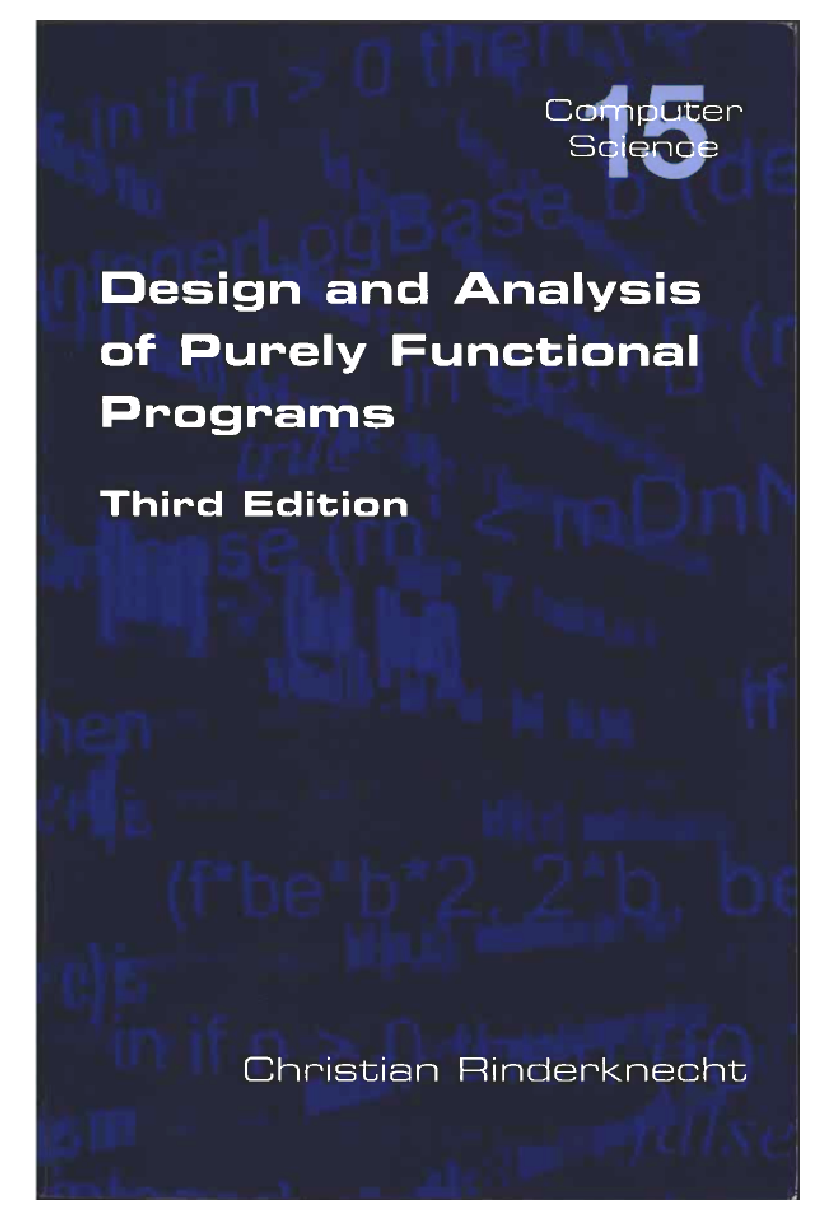
\includegraphics[scale=0.35]{my_book.eps}
  \end{minipage}%

\end{slide}

\begin{slide}
  \title{LIGO}

  \begin{itemize}

    \item At Nomadic Labs, I had two colleagues, Suzanne Dupéron and
      Gabriel Alfour.

    \item Gabriel founded a spin-off company mid-2019 and Suzanne and
      I joined him.

    \item It is funded by the Tezos Foundation to develop tools to
      ease the creation of distributed applications on Tezos.

    \item Beyond LIGO-the-language, we have produced a webIDE and a
      VSCode plug-in.

    \item The next target for LIGO-the-company is profitability.

    \item LIGO-the-company also helps with the training of Tezos
      users.

  \end{itemize}

\end{slide}

\begin{slide}
  \title{LIGO}

  \begin{itemize}

    \item Like Michelson, \textbf{LIGO is a programming language for
      writing smart contracts on Tezos.}

    \item Unlike Michelson, LIGO is a language akin to what a
      mainstream programmer would expect.

    \item This means that LIGO features variables, expressions,
      function calls, data types, pattern matching etc.

    \item Currently, LIGO is a DSL for the Tezos blockchain, but there
      is a plan to make LIGO a general-purpose language, or, at least,
      chain-agnostic.

    \item It is hosted here: \url{https://ligolang.org/}

    \item It is an \textbf{open source, collective project} (under the
      MIT licence).

    \item (If you guessed why the name ``Michelson'', you will guess
      why ``LIGO''.)

  \end{itemize}

\end{slide}

\begin{slide}
  \title{LIGO}

  \begin{itemize}

    \item Perhaps the most striking feature of LIGO is that it comes
      in \textbf{different concrete syntaxes}, and even
      \textbf{different programming paradigms}.

    \item In other words, LIGO is not defined by one syntax and one
      paradigm, like imperative versus functional.

    \item There is \textbf{PascaLIGO}, which is inspired by Pascal,
      hence is an imperative language with lots of keywords, where
      values can be locally mutated from within the scope where they
      have been declared.

    \item There is \textbf{CameLIGO}, which is inspired by the pure
      subset of OCaml, hence is a functional language with few
      keywords, where values cannot be mutated, but still require type
      annotations (unlike OCaml, whose compiler performs almost full
      type inference).

    \item There is \textbf{ReasonLIGO}, which is inspired by the pure
      subset of ReasonML, which is a JavaScript syntax on top of
      OCaml.

  \end{itemize}

\end{slide}

\begin{slide}
  \title{LIGO}

  \begin{itemize}

    \item Even within PascaLIGO, two styles are possible: terse or
      verbose. We illustrate the terse style here and in the
      documentation. We plan to offer automatic style checking and
      two-way conversion by pretty\hyp{}printing.

    \item At the call site of a function, \textbf{the arguments and
      the environment are always copied}, therefore any mutation (in
      PascaLIGO) will have no effect on the caller's arguments or the
      environment at the call site.

    \item LIGO features \textbf{higher-order functions}, that is,
      functions can be passed as arguments to others.

  \end{itemize}

\end{slide}

\begin{slide}
  \title{Tooling for LIGO}

  \begin{itemize}

    \item Several tools are currently being developed, aiming at
      facilitating the adoption of LIGO.

    \item \textbf{A VSCode plug-in} is available,
      featuring
      \begin{itemize}

        \item syntax highlighting,

        \item one-click compilation to Michelson,

        \item \emph{dry runs} to locally execute contracts on a
          sandbox.

%        \item a reactive counter estimating the gas consumption.

      \end{itemize}

    \item The architecture of VSCode, with its Language Server
      Protocol, hopefully opens the door to plugins written in any
      programming language, e.g., static analysis in OCaml.

    \item \textbf{A web-based IDE} with the same set of features.

    \item Start here: \url{https://ligolang.org/}

  \end{itemize}

\end{slide}

\begin{slide}
  \title{Research \& Development on the LIGO compiler}

  \begin{itemize}

    \item We are working on a more \textbf{powerful type system} which
      will enable the writing of more expressive contracts, featuring
      more type inference (less annotations) and enabling a greater
      variety of programming paradigms (e.g., object-oriented).

    \item We are writing a \textbf{certified backend in Coq}, that is,
      a Michelson code generator proven correct and extracted to OCaml
      from its specification.

    \item Those endeavours are not just engineering, they are
      instances of \textbf{applied research} and require a strong
      background on programming language theory.

  \end{itemize}

\end{slide}

\begin{slide}
  \title{Structure of a LIGO contract}

  \begin{itemize}

    \item A LIGO contract is a series of constant and function
      declarations.

    \item The scope of those is called \textbf{top-level}, to
      distinguish declarations that may occur within functions.

    \item In particular, even in PascaLIGO, you cannot have mutable
      variables at the top-level.

    \item As a design pattern, there is usually one special function,
      which we call \textbf{main function} that is called with a
      parameter when the contract is invoked.

    \item The main function calls other functions according to the
      value of the contract parameter.

    \item Those functions are called \textbf{entrypoints}, following
      the Michelson convention.

  \end{itemize}

\end{slide}

\begin{slide}
  \title{Constant declarations}

  \begin{itemize}

    \item LIGO lifts the basic types of Michelson, so we have
      \textsf{string}, \textsf{nat}, \textsf{int} etc.

    \item In PascaLIGO:
      \begin{alltt}
\Ktype breed \Kis string
\Kconst dog\_breed : breed = "Saluki"
      \end{alltt}

    \item In CameLIGO:
      \begin{alltt}
\Ktype breed = string
\Klet dog\_breed : breed = "Saluki"
      \end{alltt}

    \item In ReasonLIGO:
      \begin{alltt}
\Ktype breed = string;
\Klet dog\_breed : breed = "Saluki";
      \end{alltt}

  \end{itemize}

\end{slide}

\begin{slide}
  \title{Numerical Types}

  \begin{itemize}

    \item LIGO offers three built-in numerical types: \textsf{int},
      \textsf{nat} and \textsf{tez}.

    \item Literals for natural numbers are positive integers
      immediately followed by \textsf{n}, like so: \texttt{13n},
      \texttt{0n} etc.

    \item Literals for token amounts can have three forms:
      \begin{enumerate}

        \item integral amounts of tez: \texttt{2tez}, \texttt{0tez};

        \item fractional amounts of tez: \texttt{0.0003tez};

        \item integral amounts of millionth of tez:
          \texttt{340000mutez}.

      \end{enumerate}

    \item For the sake of readability, you can insert underscores to
      group digits in the integral or fractional amounts, for example
      \texttt{340\_000mutez}, or \texttt{34\_0000mutez} (in Korea), or
      \texttt{0.000\_3tez}.

    \item This also works for integers and natural numbers:
      \texttt{-10\_245}, \texttt{19\_355n}.

  \end{itemize}

\end{slide}

\begin{slide}
  \title{Addition in PascaLIGO}

  \begin{itemize}

    \item LIGO lifts the constraints of Michelson arithmetics.

      \begin{alltt}
\Kconst a : int = 5 + 10                    \com{// int + int yields int}
\Kconst b : int = 5n + 10                   \com{// nat + int yields int}
\Kconst c : tez = 5mutez + 0.000\_010tez \com{// tez + tez yields tez}

\com{// tez + int or tez + nat is invalid}
\com{// const d : tez = 5mutez + 10n}

\Kconst e : nat = 5n + 10n \com{// two nats yield a nat}

\com{// nat + int yields an int: invalid}
\com{// const f : nat = 5n + 10;}

\Kconst g : int = 1_000_000
      \end{alltt}

  \end{itemize}

\end{slide}

\begin{slide}
  \title{Addition in CameLIGO}

  \begin{itemize}

    \item LIGO lifts the constraints of Michelson arithmetics.

      \begin{alltt}
\Klet a : int = 5 + 10             \com{// int + int yields int}
\Klet b : int = 5n + 10            \com{// nat + int yields int}
\Klet c : tez = 5mutez + 10mutez \com{// tez + tez yields tez}

\com{// tez + int or tez + nat is invalid}
\com{// let d : tez = 5mutez + 10n}

\Klet e : nat = 5n + 10n \com{// two nats yield a nat}

\com{// nat + int yields an int: invalid}
\com{// let f : nat = 5n + 10}

\Klet g : int = 1_000_000
      \end{alltt}

  \end{itemize}

\end{slide}

\begin{slide}
  \title{Addition in ReasonLIGO}

  \begin{itemize}

    \item LIGO lifts the constraints of Michelson arithmetics.

      \begin{alltt}
\Klet a : int = 5 + 10;             \com{// int + int yields int}
\Klet b : int = 5n + 10;            \com{// nat + int yields int}
\Klet c : tez = 5mutez + 10mutez; \com{// tez + tez yields tez}

\com{// tez + int or tez + nat is invalid:}
\com{// let d : tez = 5mutez + 10n;}

\Klet e : nat = 5n + 10n;  \com{// two nats yield a nat}

\com{// nat + int yields an int: invalid}
\com{// let f : nat = 5n + 10;}

\Klet g : int = 1_000_000;
      \end{alltt}

  \end{itemize}

\end{slide}

\begin{slide}
  \title{Subtraction in PascaLIGO}

  \begin{itemize}

    \item LIGO lifts the constraints of Michelson arithmetics.

      \begin{alltt}
\Kconst a : int = 5 - 10

\com{// Subtraction of two nats yields an int}
\Kconst b : int = 5n - 2n

\com{// Therefore the following is invalid}
\com{// const c : nat = 5n - 2n}

\Kconst d : tez = 5mutez - 1mutez
      \end{alltt}

  \end{itemize}

\end{slide}

\begin{slide}
  \title{Subtraction in CameLIGO}

  \begin{itemize}

    \item LIGO lifts the constraints of Michelson arithmetics.

      \begin{alltt}
\Klet a : int = 5 - 10

\com{// Subtraction of two nats yields an int}
\Klet b : int = 5n - 2n

\com{// Therefore the following is invalid}
\com{// let c : nat = 5n - 2n}

\Klet d : tez = 5mutez - 1mutez
      \end{alltt}

  \end{itemize}

\end{slide}

\begin{slide}
  \title{Subtraction in ReasonLIGO}

  \begin{itemize}

    \item LIGO lifts the constraints of Michelson arithmetics.

      \begin{alltt}
\Klet a : int = 5 - 10;

\com{// Subtraction of two nats yields an int}
\Klet b : int = 5n - 2n;

\com{// Therefore the following is invalid}
\com{// let c : nat = 5n - 2n;}

\Klet d : tez = 5mutez - 1mutez;
      \end{alltt}

  \end{itemize}

\end{slide}

\begin{slide}
  \title{Multiplication and Division in PascaLIGO}

  \begin{itemize}

    \item LIGO lifts the constraints of Michelson arithmetics.

      \begin{alltt}
\Kconst a : int = 5 * 5
\Kconst b : nat = 5n * 5n
\Kconst c : tez = 5n * 5mutez \com{// You can also multiply nat and tez}

\Kconst d : int = 10 / 3
\Kconst e : nat = 10n / 3n
\Kconst f : nat = 10mutez / 3mutez
      \end{alltt}

  \end{itemize}

\end{slide}

\begin{slide}
  \title{Multiplication and Division in CameLIGO}

  \begin{itemize}

    \item LIGO lifts the constraints of Michelson arithmetics.

      \begin{alltt}
\Klet a : int = 5 * 5
\Klet b : nat = 5n * 5n
\Klet c : tez = 5n * 5mutez \com{// You can also multiply nat and tez}

\Klet d : int = 10 / 3
\Klet e : nat = 10n / 3n
\Klet f : nat = 10mutez / 3mutez
      \end{alltt}

  \end{itemize}

\end{slide}

\begin{slide}
  \title{Multiplication and Division in ReasonLIGO}

  \begin{itemize}

    \item LIGO lifts the constraints of Michelson arithmetics.

      \begin{alltt}
\Klet a : int = 5 * 5;
\Klet b : nat = 5n * 5n;
\Klet c : tez = 5n * 5mutez; \com{// You can also multiply nat and tez}

\Klet d : int = 10 / 3;
\Klet e : nat = 10n / 3n;
\Klet f : nat = 10mutez / 3mutez;
      \end{alltt}
  \end{itemize}

\end{slide}

\begin{slide}
  \title{Casts}

  \begin{itemize}

    \item You can \textbf{cast} an \textsf{int} to a \textsf{nat} and
      vice versa.

    \item In PascaLIGO:
      \begin{alltt}
\Kconst a : int = int (1n)
\Kconst b : nat = abs (1)
      \end{alltt}

    \item In CameLIGO:
      \begin{alltt}
\Klet a : int = int (1n)
\Klet b : nat = abs (1)
      \end{alltt}

    \item In ReasonLIGO:
      \begin{alltt}
\Klet a : int = int (1n);
\Klet b : nat = abs (1);
      \end{alltt}
  \end{itemize}

\end{slide}

\begin{slide}
  \title{Checks}

  \begin{itemize}

    \item You can check if a value is a \textsf{nat} by using a
      predefined cast function which accepts an \textsf{int} and
      returns an optional \textsf{nat}: if the result is not
      \textsf{None}, then the provided integer was indeed a natural
      number, and not otherwise.

    \item We will revisit this when we present the \textbf{variant}
      types.

      \item In PascaLIGO:
        \begin{alltt}
\Kconst is_a_nat : option (nat) = is_nat (1)
        \end{alltt}

      \item In CameLIGO:
        \begin{alltt}
\Klet is_a_nat : nat option = is_nat (1)
        \end{alltt}

      \item In ReasonLIGO:
        \begin{alltt}
\Klet is_a_nat : option (nat) = is_nat (1);
        \end{alltt}

  \end{itemize}

\end{slide}

\begin{slide}
  \title{Strings}

  \begin{itemize}

    \item In PascaLIGO:
      \begin{alltt}
\Kconst name : string = "Alice"
\Kconst greeting : string = "Hello"
\Kconst full_greeting : string = greeting ^ " " ^ name
      \end{alltt}

    \item In CameLIGO:
      \begin{alltt}
\Klet name : string = "Alice"
\Klet greeting : string = "Hello"
\Klet full_greeting : string = greeting ^ " " ^ name
      \end{alltt}

    \item In ReasonLIGO:
      \begin{alltt}
\Klet name : string = "Alice";
\Klet greeting : string = "Hello";
\Klet full_greeting : string = greeting ++ " " ++ name;
      \end{alltt}

  \end{itemize}

\end{slide}

\begin{slide}
  \title{Booleans}

  \begin{itemize}

    \item The type of the booleans is \texttt{bool}.

    \item In PascaLIGO:
      \begin{alltt}
\Kconst a : bool = \KTrue   \com{// \Ktrue also}
\Kconst b : bool = \KFalse  \com{// \Kfalse also}
      \end{alltt}

    \item In CameLIGO:
      \begin{alltt}
\Klet a : bool = \Ktrue
\Klet b : bool = \Kfalse
      \end{alltt}

    \item In ReasonLIGO:
      \begin{alltt}
\Klet a : bool = \Ktrue;
\Klet b : bool = \Kfalse;
      \end{alltt}

  \end{itemize}

\end{slide}

\begin{slide}
  \title{Comparing Values}

  \begin{itemize}

    \item In LIGO, only values of the same type can be
      compared. Moreover, not all values of the same type can be
      compared, only those with \textbf{comparable types}, which is a
      concept lifted from Michelson.

    \item Comparable types include, for instance, \texttt{int},
      \texttt{nat}, \texttt{string}, \texttt{tez}, \texttt{timestamp},
      \texttt{address}, etc. As an example of non-comparable types:
      maps, sets or lists are not comparable: if you wish to compare
      them, you will have to write your own comparison function.

  \end{itemize}

\end{slide}

\begin{slide}
  \title{Comparing Strings}

  \begin{itemize}

    \item In PascaLIGO:
      \begin{alltt}
\Kconst a : string = "Alice"
\Kconst b : string = "Alice"
\Kconst c : bool = (a = b) \com{// \KTrue}
      \end{alltt}

    \item In CameLIGO:
      \begin{alltt}
\Klet a : string = "Alice"
\Klet b : string = "Alice"
\Klet c : bool = (a = b) \com{// \Ktrue}
      \end{alltt}

    \item In ReasonLIGO:
      \begin{alltt}
\Klet a : string = "Alice";
\Klet b : string = "Alice";
\Klet c : bool = (a == b); \com{// \Ktrue}
      \end{alltt}

  \end{itemize}

\end{slide}

\begin{slide}
  \title{Comparing Numbers in PascaLIGO}

      \begin{alltt}
\Kconst a : int  = 5
\Kconst b : int  = 4
\Kconst c : bool = (a = b)
\Kconst d : bool = (a > b)
\Kconst e : bool = (a < b)
\Kconst f : bool = (a <= b)
\Kconst g : bool = (a >= b)
\Kconst h : bool = (a =/= b)
      \end{alltt}

\end{slide}

\begin{slide}
  \title{Comparing Numbers in CameLIGO}

      \begin{alltt}
\Klet a : int  = 5
\Klet b : int  = 4
\Klet c : bool = (a = b)
\Klet d : bool = (a > b)
\Klet e : bool = (a < b)
\Klet f : bool = (a <= b)
\Klet g : bool = (a >= b)
\Klet h : bool = (a <> b)
      \end{alltt}

\end{slide}

\begin{slide}
  \title{Comparing Numbers in ReasonLIGO}

      \begin{alltt}
\Klet a : int  = 5;
\Klet b : int  = 4;
\Klet c : bool = (a == b);
\Klet d : bool = (a > b);
\Klet e : bool = (a < b);
\Klet f : bool = (a <= b);
\Klet g : bool = (a >= b);
\Klet h : bool = (a != b);
      \end{alltt}

\end{slide}

\begin{slide}
  \title{Tuples}

  \begin{itemize}

    \item Tuples gather a given number of values in a specific order
      and those values, called \textbf{components}, can be retrieved
      by their index (position).

    \item Probably the most common tuple is the \textbf{pair}. For
      example, if we were storing coordinates on a two dimensional
      grid we might use a pair \texttt{(x,y)} to store the coordinates
      \texttt{x} and \texttt{y}.

    \item There is a \textbf{specific order}, so \texttt{(y,x)} is not
      equal to \texttt{(x,y)} in general.

    \item The number of components is part of the type of a tuple, so,
      for example, we cannot add an extra component to a pair and
      obtain a triple of the same type: \texttt{(x,y)} has always a
      different type from \texttt{(x,y,z)}, whereas \texttt{(y,x)}
      might have the same type as \texttt{(x,y)}.

    \item Like record fields, tuple components can be of arbitrary
      types.

  \end{itemize}

\end{slide}

\begin{slide}
  \title{Tuple Definition}

  \begin{itemize}

    \item Unlike a record, tuple types do not have to be defined
      before they can be used. However below we will give them names
      by \textbf{type aliasing}.

    \item In PascaLIGO:
      \begin{alltt}
\Ktype full_name is string * string  \com{// Alias}
\Kconst full_name : full_name = ("Alice", "Johnson")
      \end{alltt}

    \item In CameLIGO:
      \begin{alltt}
\Ktype full_name = string * string  \com{// Alias}
\com{// Optional parentheses:}
\Klet full_name : full_name = ("Alice", "Johnson")
      \end{alltt}

    \item In ReasonLIGO:
      \begin{alltt}
\Ktype full_name = (string, string);  \com{// Alias}
\Klet full_name : full_name = ("Alice", "Johnson");
      \end{alltt}

  \end{itemize}

\end{slide}

\begin{slide}
  \title{Accessing Tuple Components}

  \begin{itemize}

    \item Accessing the components of a tuple in OCaml is achieved by
      \textbf{pattern matching}. LIGO currently supports tuple
      patterns only in the parameters of functions, not in pattern
      matching. However, we can access components by their position in
      their tuple, which cannot be done in OCaml. Components are
      zero-indexed, that is, the first has index~\(0\).

    \item In PascaLIGO:
      \begin{alltt}
\Kconst first_name : string = full_name.0
      \end{alltt}

    \item In CameLIGO:
      \begin{alltt}
\Klet first_name : string = full_name.0
      \end{alltt}

    \item In ReasonLIGO:
      \begin{alltt}
\Klet first_name : string = full_name[0];
      \end{alltt}

  \end{itemize}

\end{slide}

\begin{slide}
  \title{Lists}

  \begin{itemize}

    \item Lists are linear collections of elements of the same
      type. Linear means that, in order to reach an element in a list,
      we must visit all the elements before (sequential
      access).

    \item Elements can be repeated, as only their order in the
      collection matters. The first element is called the
      \textbf{head}, and the sub-list after the head is called the
      \textbf{tail}.

    \item For those familiar with algorithmic data structure, you can
      think of a list a \textbf{stack}, where the top is written on
      the left.

    \item Lists are needed when returning operations from a smart
      contract's main function.

  \end{itemize}

\end{slide}


\begin{slide}
  \title{Defining Lists}

  \begin{itemize}

    \item In PascaLIGO:
      \begin{alltt}
\Kconst empty_list : list (int) = \Knil          \com{// Or: list []}
\Kconst my_list : list (int) = \Klist [1; 2; 2] \com{// The head is 1}
      \end{alltt}

    \item In CameLIGO:
      \begin{alltt}
\Klet empty_list : int list = []
\Klet my_list : int list = [1; 2; 2] \com{// The head is 1}
      \end{alltt}

    \item In ReasonLIGO:
      \begin{alltt}
\Klet empty_list : list (int) = [];
\Klet my_list : list (int) = [1, 2, 2]; \com{// The head is 1}
      \end{alltt}

  \end{itemize}

\end{slide}

\begin{slide}
  \title{Adding to Lists}

  \begin{itemize}

    \item Lists can be augmented by adding an element before the head
      (or, in terms of stack, by \textbf{pushing an element on
      top}). This operation is usually called \textbf{consing} in
      functional languages.

    \item In PascaLIGO, the \textbf{cons operator} is infix and noted
      \texttt{\#}. It is not symmetric: on the left lies the element to
      cons, and, on the right, a list on which to cons. (The symbol is
      helpfully asymmetric to remind you of that.)
      \begin{alltt}
\Kconst larger_list : list (int) = 5 \# my_list \com{// [5;1;2;2]}
      \end{alltt}

  \end{itemize}

\end{slide}

\begin{slide}
  \title{Adding to Lists}

  \begin{itemize}

    \item In CameLIGO, the \textbf{cons operator} is infix and noted
      \texttt{::}. It is not symmetric: on the left lies the element
      to cons, and, on the right, a list on which to cons.
      \begin{alltt}
\Klet larger_list : int list = 5 :: my_list \com{// [5;1;2;2]}
      \end{alltt}

    \item In ReasonLIGO, the \textbf{cons operator} is infix and noted
      ``\texttt{, ...}''. It is not symmetric: on the left lies the
      element to cons, and, on the right, a list on which to cons.
      \begin{alltt}
\Klet larger_list : list (int) = [5, ...my_list]; \com{// [5,1,2,2]}
      \end{alltt}

  \end{itemize}

\end{slide}

\begin{slide}
  \title{Sets}

  \begin{itemize}

    \item Sets are unordered collections of values of the same type,
      like lists are ordered collections. Like the mathematical sets
      and lists, sets can be empty and, if not, elements of sets in
      LIGO are \textbf{unique}, whereas they can be repeated in a
      list.

    \item In PascaLIGO, the notation for sets is similar to that for
      lists, except the keyword \textbf{set} is used before:
      \begin{alltt}
\Kconst my_set : set (int) = \Kset []
      \end{alltt}

    \item In CameLIGO, the empty set is denoted by the predefined
      value \texttt{Set.empty}:
      \begin{alltt}
\Klet my_set : int set = Set.empty
      \end{alltt}

    \item In ReasonLIGO, the empty set is denoted by the predefined
      value \texttt{Set.empty}:
      \begin{alltt}
\Klet my_set : set (int) = Set.empty;
      \end{alltt}

  \end{itemize}

\end{slide}

\begin{slide}
  \title{Adding to Sets}

  \begin{itemize}

    \item In PascaLIGO, the notation for non-empty sets follows that
      for lists:
      \begin{alltt}
\Kconst my_set : set (int) = \Kset [3; 2; 2; 1]
      \end{alltt}

    \item In CameLIGO, to add to a set, use the predefined function
      \texttt{Set.add}:
      \begin{alltt}
\Klet my_set : int set =
  Set.add 3 (Set.add 2 (Set.add 2 (Set.add 1 (Set.empty : int set))))
      \end{alltt}

    \item In ReasonLIGO, to add to a set, use the predefined function
      \texttt{Set.add}:
      \begin{alltt}
\Klet my_set : set (int) =
  Set.add (3,
             Set.add (2,
                        Set.add (2,
                                   Set.add (1, Set.empty : set (int)))));
      \end{alltt}

  \end{itemize}

\end{slide}

\begin{slide}
  \title{Set Membership}

  \begin{itemize}

    \item PascaLIGO features a special keyword
      \textbf{\texttt{contains}} that operates like an infix operator
      checking membership in a set:
      \begin{alltt}
\Kconst contains_3 : bool = my_set \Kcontains 3
      \end{alltt}

    \item In CameLIGO, the predefined predicate \texttt{Set.mem} tests
      for membership in a set as follows:
      \begin{alltt}
\Klet contains_3 : bool = Set.mem 3 my_set
      \end{alltt}

    \item In ReasonLIGO, the predicate is \texttt{Set.mem} as well:
      \begin{alltt}
\Klet contains_3 : bool = Set.mem (3, my_set);
      \end{alltt}

  \end{itemize}

\end{slide}

\begin{slide}
  \title{Cardinal}

  \begin{itemize}

    \item In PascaLIGO, the predefined function \texttt{size} returns
      the number of elements in a given set as follows:
      \begin{alltt}
\Kconst set_size : nat = Set.size (my_set)
      \end{alltt}

    \item In CameLIGO, the predefined function \texttt{Set.size}
      returns the number of elements in a given set as follows:
      \begin{alltt}
\Klet set_size : nat = Set.size my_set
      \end{alltt}

    \item In ReasonLIGO, the predefined function is \texttt{Set.size}
      too:
      \begin{alltt}
\Klet set_size : nat = Set.size (my_set);
      \end{alltt}

  \end{itemize}

\end{slide}


\begin{slide}
  \title{Updating Sets in PascaLIGO}

  \begin{itemize}

    \item In PascaLIGO, there are two ways to update a set, that is to
      add or remove from it. Either we create a new set from the given
      one, or we modify it in-place. First, let us consider the former
      way:
      \begin{alltt}
\Kconst larger_set  : set (int) = Set.add (4, my_set)
\Kconst smaller_set : set (int) = Set.remove (3, my_set)
      \end{alltt}

    \item If we are in a block, we can use an instruction to modify
      the set bound to a given variable. This is called a
      \textbf{patch}. It is only possible to add elements by means of
      a patch, not remove any: it is the union of two sets.
      \begin{alltt}
\Kfunction update (\Kvar s : set (int)) : set (int) \Kis \Kblock \{
  \Kpatch s \Kwith \Kset [4; 7]
\} \Kwith s

\Kconst new_set : set (int) = update (my_set)
      \end{alltt}

  \end{itemize}

\end{slide}

\begin{slide}
  \title{Updating Sets in CameLIGO and ReasonLIGO}

  \begin{itemize}

    \item In CameLIGO, we update a given set by creating another one,
      with or without some elements:
      \begin{alltt}
\Klet larger_set  : int set = Set.add 4 my_set
\Klet smaller_set : int set = Set.remove 3 my_set
      \end{alltt}

    \item In ReasonLIGO, the update is similar to CameLIGO:
      \begin{alltt}
\Klet larger_set  : set (int) = Set.add (4, my_set);
\Klet smaller_set : set (int) = Set.remove (3, my_set);
      \end{alltt}

  \end{itemize}

\end{slide}


\begin{slide}
  \title{Functions in PascaLIGO}

  \begin{itemize}

    \item LIGO functions are the basic building block of
      contracts. For example, entrypoints are functions.

    \item There are two ways in PascaLIGO to define functions: with or
      without a \textbf{block}.

    \item Blocks enable the sequential composition of instructions
      into an isolated scope. Each block needs to include at least one
      instruction.
      \begin{alltt}
\Kblock \{ a := a + 1 \}
      \end{alltt}

    \item If we need a placeholder, we use the instruction \Kskip
      which leaves the state unchanged.  The rationale for \Kskip
      instead of a truly empty block is that it prevents you from
      writing an empty block by mistake.
      \begin{alltt}
\Kblock \{ \Kskip \}
      \end{alltt}

    \item Blocks are more versatile than simply containing
      instructions: they can also include \textbf{declarations} of
      values, like so:
      \begin{alltt}
\Kblock \{ \Kconst a : int = 1 \}
      \end{alltt}

  \end{itemize}

\end{slide}

\begin{slide}
  \title{Block-based Functions in PascaLIGO}

  \begin{itemize}

    \item Functions in PascaLIGO are defined using the \Kfunction
      keyword followed by their \textbf{name}, \textbf{parameters} and
      \textbf{return} type definitions.

    \item Here is how you define a basic function that computes the
      sum of two integers:
      \begin{alltt}
\Kfunction add (\Kconst a : int; \Kconst b : int) : int \Kis
  \Kblock \{
    \Kconst c : int = a + b
  \} \Kwith c
      \end{alltt}

  \item The function body consists of two parts:
    \begin{enumerate}

      \item \texttt{\Kblock \{ <instructions and declarations> \}} is
        the logic of the function;

      \item \texttt{\Kwith <value>} is the value returned by the
        function.

    \end{enumerate}

  \end{itemize}

\end{slide}


\begin{slide}
  \title{Blockless Functions in PascaLIGO}

  \begin{itemize}

    \item Functions that can contain all of their logic into a single
      \textbf{expression} can be defined without the need of a block:
      \begin{alltt}
\com{// Bad! Empty block not needed!}
\Kfunction identity (\Kconst n : int) : int \Kis \Kblock \{ \Kskip \} \Kwith n

\com{// Better}
\Kfunction identity (\Kconst n : int) : int \Kis n  \com{// Blockless}
      \end{alltt}

    \item The value of the expression is implicitly returned by the
      function.
      \begin{alltt}
\Kfunction add (\Kconst a: int; \Kconst b : int) : int \Kis a + b
      \end{alltt}

  \end{itemize}

\end{slide}

\begin{slide}
  \title{Functions in CameLIGO}

  \begin{itemize}

    \item Functions in CameLIGO are defined using the \Klet keyword,
      like other values. The difference is that a succession of
      parameters is provided after the value name, followed by the
      return type. This follows OCaml syntax.
      \begin{alltt}
\Klet add (a : int) (b : int) : int = a + b
      \end{alltt}

    \item CameLIGO is a little different from other syntaxes when it
      comes to function parameters. In OCaml, functions can only take
      one parameter. To get functions with multiple arguments like we
      are used to in imperative programming languages, a technique
      called \textbf{currying} is used.

  \end{itemize}

\end{slide}

\begin{slide}
  \title{Functions in CameLIGO}

  \begin{itemize}

    \item Currying essentially translates a function with multiple
      arguments into a series of single argument functions, each
      returning a new function accepting the next argument until every
      parameter is filled. This is useful because it means that
      CameLIGO supports \textbf{partial application}.

    \item Currying is however \textbf{not} the preferred way to pass
      function arguments in CameLIGO.  While this approach is faithful
      to the original OCaml, it is costlier in Michelson than naive
      function execution accepting multiple arguments. Instead, for
      most functions with more than one parameter, we should gather
      the arguments in a \textbf{tuple} and pass the tuple in as a
      single parameter.

    \item Here is how you define a basic function that accepts two
      integers and returns an integer as well:
      \begin{alltt}
\Klet add (a, b : int * int) : int = a + b \com{// Uncurried}
\Klet add\_curry (a : int) (b : int) : int = add (a, b) \com{// Curried}
\Klet increment (b : int) : int = add\_curry 1 \com{// Partial application}
      \end{alltt}

    \item The function body is a single expression, whose value is
      returned.

  \end{itemize}

\end{slide}

\begin{slide}
  \title{Functions in ReasonLIGO}

  \begin{itemize}

    \item Functions in ReasonLIGO are defined using the \Klet keyword,
      like other values. The difference is that a tuple of parameters
      is provided after the value name, with its type, then followed
      by the return type.

    \item Here is how you define a basic function that sums two
      integers:
      \begin{alltt}
\Klet add = ((a, b): (int, int)) : int => a + b;
      \end{alltt}

      \item As in CameLIGO and with blockless functions in PascaLIGO,
        the function body is a single expression, whose value is
        returned.

      \item If the body contains more than a single expression, you
        use a \textbf{block} between braces:
        \begin{alltt}
\Klet myFun = ((x, y) : (int, int)) : int =>
\{
  \Klet doubleX = x + x;
  \Klet doubleY = y + y;
  doubleX + doubleY
\};
        \end{alltt}

  \end{itemize}

\end{slide}

\begin{slide}
  \title{Anonymous functions (a.k.a. lambdas)}

  \begin{itemize}

    \item It is possible to define functions without assigning them a
      name. They are useful when you want to pass them as arguments,
      or assign them to a key in a record or a map.

    \item In PascaLIGO:
      \begin{alltt}
\Kfunction increment (\Kconst b : int) : int is
   (\Kfunction (\Kconst a : int) : int is a + 1) (b)
\Kconst a : int = increment (1); // a = 2
      \end{alltt}

    \item In CameLIGO:
      \begin{alltt}
\Klet increment (b : int) : int = (\Kfun (a : int) -> a + 1) b
\Klet a : int = increment 1 // a = 2
      \end{alltt}

    \item In ReasonLIGO:
      \begin{alltt}
\Klet increment = (b : int) : int => ((a : int) : int => a + 1) (b);
\Klet a : int = increment (1); // a == 2
      \end{alltt}
  \end{itemize}

\end{slide}


\begin{slide}
  \title{Anonymous functions (a.k.a. lambdas)}

  \begin{itemize}

    \item If the example above seems contrived, here is a more common
      design pattern for lambdas: to be used as parameters to
      functions. Consider the use case of having a list of integers
      and mapping the increment function to all its elements.

    \item In PascaLIGO:
      \begin{alltt}
\Kfunction incr_map (\Kconst l : list (int)) : list (int) \Kis
  List.map (\Kfunction (\Kconst i : int) : int \Kis i + 1, l)
      \end{alltt}

    \item In CameLIGO:
      \begin{alltt}
\Klet incr_map (l : int list) : int list =
  List.map (\Kfun (i : int) -> i + 1) l
      \end{alltt}

    \item In ReasonLIGO:
      \begin{alltt}
\Klet incr_map = (l : list (int)) : list (int) =>
  List.map ((i : int) => i + 1, l);
      \end{alltt}
  \end{itemize}

\end{slide}

\begin{slide}
  \title{The unit Type}

  \begin{itemize}

    \item The \texttt{unit} type in Michelson or LIGO is a predefined
      type that contains only one value that carries no
      information. It is used when no relevant information is required
      or produced.

    \item In PascaLIGO, the unique value of the \texttt{unit} type is
      \KUnit:
      \begin{alltt}
\Kconst n : unit = \KUnit \com{// Or unit}
      \end{alltt}

    \item In CameLIGO, the unique value of the \texttt{unit} type is
      \texttt{()}, following the OCaml convention:
      \begin{alltt}
\Klet n : unit = ()
      \end{alltt}

    \item In ReasonLIGO, the unique value of the \texttt{unit} type is
      \texttt{()}, following the ReasonML convention:
      \begin{alltt}
\Klet n : unit = ();
      \end{alltt}

  \end{itemize}

\end{slide}

\begin{slide}
  \title{Functional Iterations over Lists}

  \begin{itemize}

    \item A \textbf{functional iterator} is a function that traverses
      a data structure and calls in turn a given function over the
      elements of that structure to compute some value. (Another
      approach is possible in PascaLIGO: \textbf{loops}.)

    \item There are three kinds of functional iterations over LIGO
      lists:
      \begin{enumerate}

        \item the \textbf{iterated operation},

        \item the \textbf{mapped operation} (not to be
          confused with the \emph{map data structure}),

        \item and the \textbf{folded operation}.

      \end{enumerate}

  \end{itemize}

\end{slide}

\begin{slide}
  \title{Iterated Operations over Lists}

  \begin{itemize}

    \item The first, the \textbf{iterated operation}, is an iteration
      over the list with a unit return value. It is useful to enforce
      certain invariants on the element of a list, or fail. For
      example you might want to check that each value inside of a list
      is within a certain range, and fail otherwise.

    \item In PascaLIGO, the predefined functional iterator
      implementing the iterated operation over lists is called
      \texttt{List.iter}.

    \item In the following example, a list is iterated to check that
      all its elements (integers) are greater than~\(3\):
      \begin{alltt}
\Kfunction iter_op (\Kconst l : list (int)) : unit \Kis
  \Kblock \{
    \Kfunction iterated (\Kconst i : int) : unit \Kis
      \Kif i > 3 \Kthen \KUnit \Kelse (failwith ("Below range.") : unit)
  \} \Kwith List.iter (iterated, l)
      \end{alltt}

  \end{itemize}

\end{slide}

\begin{slide}
  \title{Iterated Operations over Lists}

  \begin{itemize}

    \item In CameLIGO, the predefined functional iterator implementing
      the iterated operation over lists is called \texttt{List.iter}.
      \begin{alltt}
\Klet iter_op (l : int list) : unit =
  \Klet predicate = \Kfun (i : int) -> assert (i > 3)
  \Kin List.iter predicate l
      \end{alltt}

    \item In ReasonLIGO, the predefined functional iterator
      implementing the iterated operation over lists is also called
      \texttt{List.iter}:
      \begin{alltt}
\Klet iter_op = (l : list (int)) : unit => \{
  \Klet predicate = (i : int) => assert (i > 3);
  List.iter (predicate, l);
\};
      \end{alltt}

  \end{itemize}

\end{slide}

\begin{slide}
  \title{Map Operations over Lists}

  \begin{itemize}

    \item We may want to change all the elements of a given list by
      applying to them a function. This is called a \textbf{map
        operation}, not to be confused with the map data structure.

    \item In PascaLIGO, the predefined functional iterator
      implementing the map operation over lists is called
      \texttt{List.map}:
      \begin{alltt}
\Kfunction increment (\Kconst i : int): int \Kis i + 1
\com{// Creates a new list with all elements incremented by 1}
\Kconst plus_one : list (int) = List.map (increment, larger_list)
      \end{alltt}

    \item In CameLIGO, the predefined functional iterator implementing
      the map operation over lists is called \texttt{List.map}:
      \begin{alltt}
\Klet increment (i : int) : int = i + 1
\com{// Creates a new list with all elements incremented by 1}
\Klet plus_one : int list = List.map increment larger_list
      \end{alltt}

  \end{itemize}

\end{slide}

\begin{slide}
  \title{Map Operations over Lists}

  \begin{itemize}

    \item In ReasonLIGO, the predefined functional iterator
      implementing the map operation over lists is called
      \texttt{List.map}:
      \begin{alltt}
\Klet increment = (i : int) : int => i + 1;
\com{// Creates a new list with all elements incremented by 1}
\Klet plus_one : list (int) = List.map (increment, larger_list);
      \end{alltt}

  \end{itemize}

\end{slide}

\begin{slide}
  \title{Folded Operations over Lists}

  \begin{itemize}

    \item A \textbf{folded operation} is the most general of
      iteration. The folded function takes two arguments: an
      \textbf{accumulator} and the structure \textbf{element} at hand,
      with which it then produces a new accumulator. This enables
      having a partial result that becomes complete when the traversal
      of the data structure is over.

    \item In PascaLIGO, the predefined functional iterator
      implementing the folded operation over lists is called
      \texttt{List.fold}:
      \begin{alltt}
\Kfunction sum (\Kconst acc : int; \Kconst i : int): int \Kis acc + i
\Kconst sum_of_elements : int = List.fold (sum, my_list, 0)
      \end{alltt}

  \end{itemize}

\end{slide}

\begin{slide}
  \title{Folded Operations over Lists}

  \begin{itemize}

    \item In CameLIGO, the predefined functional iterator implementing
      the folded operation over lists is called \texttt{List.fold}:
      \begin{alltt}
\Klet sum (acc, i: int * int) : int = acc + i
\Klet sum_of_elements : int = List.fold sum my_list 0
      \end{alltt}

    \item In ReasonLIGO, the name of the iterator is also
      \texttt{List.fold}:
      \begin{alltt}
\Klet sum = ((result, i): (int, int)): int => result + i;
\Klet sum_of_elements : int = List.fold (sum, my_list, 0);
      \end{alltt}

  \end{itemize}

\end{slide}

\begin{slide}
  \title{Functional Iterations over Sets}

  \begin{itemize}

  \item Like for lists, there are three kinds of functional iterations
    over LIGO sets:
      \begin{enumerate}

        \item the \textbf{iterated operation},

        \item the \textbf{mapped operation} (not to be
          confused with the *map data structure*),

        \item and the \textbf{folded operation}.

      \end{enumerate}

  \end{itemize}

\end{slide}

\begin{slide}
  \title{Iterated Operations over Sets}

  \begin{itemize}

    \item In PascaLIGO, the predefined functional iterator
      implementing the iterated operation over sets is called
      \texttt{Set.iter}.

    \item In the following example, a set is iterated to check that
      all its elements (integers) are greater than~\(3\):
      \begin{alltt}
\Kfunction iter_op (\Kconst s : set (int)) : unit \Kis
  \Kblock \{
    \Kfunction iterated (const i : int) : unit \Kis
      \Kif i > 3 \Kthen \KUnit \Kelse (failwith ("Below range.") : unit)
  \} \Kwith Set.iter (iterated, s)
      \end{alltt}

  \end{itemize}

\end{slide}

\begin{slide}
  \title{Iterated Operations over Sets}

  \begin{itemize}

    \item In CameLIGO, the predefined functional iterator implementing
      the iterated operation over sets is called \texttt{Set.iter}.
      \begin{alltt}
\Klet iter_op (s : int set) : unit =
  \Klet predicate = \Kfun (i : int) -> assert (i > 3)
  \Kin Set.iter predicate s
      \end{alltt}

    \item In ReasonLIGO, the predefined functional iterator implementing
      the iterated operation over sets is called \texttt{Set.iter}
      too.
      \begin{alltt}
\Klet iter_op = (s : set (int)) : unit => \{
  \Klet predicate = (i : int) => assert (i > 3);
  Set.iter (predicate, s);
\};
      \end{alltt}

  \end{itemize}

\end{slide}

\begin{slide}
  \title{Folded Operations over Sets}

  \begin{itemize}

    \item In PascaLIGO, the predefined functional iterator
      implementing the folded operation over sets is called
      \texttt{Set.fold}.
      \begin{alltt}
\Kfunction sum (\Kconst acc : int; \Kconst i : int): int \Kis acc + i
\Kconst sum_of_elements : int = Set.fold (sum, my_set, 0)
      \end{alltt}

    \item In CameLIGO, the predefined fold over sets is called
      \texttt{Set.fold}:
      \begin{alltt}
\Klet sum (acc, i : int * int) : int = acc + i
\Klet sum_of_elements : int = Set.fold sum my_set 0
      \end{alltt}

    \item In ReasonLIGO, the predefined fold over sets is called
      \texttt{Set.fold} as well:
      \begin{alltt}
\Klet sum = ((acc, i) : (int, int)) : int => acc + i;
\Klet sum_of_elements : int = Set.fold (sum, my_set, 0);
      \end{alltt}

  \end{itemize}

\end{slide}

\begin{slide}
  \title{Variant Types}

  \begin{itemize}

    \item A variant type is a user-defined or a built-in type (in case
      of options) that defines a type by cases, so a value of a
      variant type is either this, or that or... and nothing else. The
      simplest variant type is equivalent to the enumerated types
      found in Java.

    \item In PascaLIGO:
      \begin{alltt}
\Ktype coin \Kis Head | Tail
\Kconst head : coin = Head \com{// Equivalent to Head (Unit)}
\Kconst tail : coin = Tail \com{// Equivalent to Tail (Unit)}
      \end{alltt}

      \vspace{-5mm}
    \item In CameLIGO:
      \begin{alltt}
\Ktype coin = Head | Tail
\Klet head : coin = Head
\Klet tail : coin = Tail
      \end{alltt}

      \vspace{-5mm}
    \item In ReasonLIGO:
      \begin{alltt}
\Ktype coin = Head | Tail;
\Klet head : coin = Head;
\Klet tail : coin = Tail;
      \end{alltt}

  \end{itemize}

\end{slide}

\begin{slide}
  \title{Variant Types}

  \begin{itemize}

    \item The names \texttt{Head} and \texttt{Tail} in the definition
      of the type \texttt{coin} are called \textbf{data constructors},
      or \textbf{variants}.

    \item In general, it is interesting for variants to carry some
      information, and thus go beyond enumerated types.

    \item In the following, we show how to define different kinds of
      users of a system.

  \end{itemize}

\end{slide}

\begin{slide}
  \title{Variants in PascaLIGO}

\begin{alltt}
\Ktype id \Kis nat

\Ktype user \Kis
  Admin   \Kof id
| Manager \Kof id
| Guest

\Kconst u : user = Admin (1000n)
\Kconst g : user = Guest         \com{// Equivalent to Guest (Unit)}
\end{alltt}

\end{slide}

\begin{slide}
  \title{Variants in CameLIGO}

\begin{alltt}
\Ktype id = nat

\Ktype user =
  Admin   \Kof id
| Manager \Kof id
| Guest

\Klet u : user = Admin 1000n
\Klet g : user = Guest
\end{alltt}

\end{slide}

\begin{slide}
  \title{Variants in ReasonLIGO}

\begin{alltt}
\Ktype id = nat;

\Ktype user =
| Admin   (id)
| Manager (id)
| Guest;

\Klet u : user = Admin (1000n);
\Klet g : user = Guest;
\end{alltt}

\end{slide}

\begin{slide}
  \title{Conditionals}

  \begin{itemize}

    \item Conditional logic enables forking the control flow depending
      on the state.

    \item In PascaLIGO:
      \begin{alltt}
\Ktype magnitude \Kis Small | Large
\Kfunction compare (\Kconst n : nat) : magnitude \Kis
  \Kif n < 10n \Kthen Small \Kelse Large
      \end{alltt}

    \item In CameLIGO:
      \begin{alltt}
\Ktype magnitude = Small | Large
\Klet compare (n : nat) : magnitude = \Kif n < 10n \Kthen Small \Kelse Large
      \end{alltt}

    \item In ReasonLIGO:
      \begin{alltt}
\Ktype magnitude = Small | Large;
\Klet compare = (n : nat) : magnitude =>
  \Kif (n < 10n) \{ Small; \} \Kelse \{ Large; \};
      \end{alltt}

  \end{itemize}

\end{slide}

\begin{slide}
  \title{Conditionals}

  \begin{itemize}

    \item When the branches of the conditional are not a single
      expression, as above, we need a block:
      \begin{alltt}
\Kif x < y \Kthen
  \Kblock \{
    \Kconst z : nat = x;
    x := y; y := z
  \}
  \Kelse \Kskip;
      \end{alltt}

    \item As an exception to the rule, the blocks in a conditional
      branch do not need to be introduced by the keyword \Kblock, so,
      we could have written instead:
\begin{alltt}
\Kif x < y \Kthen \{
  \Kconst z : nat = x;
  x := y; y := z
\}
\Kelse \Kskip;
\end{alltt}

  \end{itemize}

\end{slide}

\begin{slide}
  \title{Conditionals}

  \begin{itemize}

    \item Like in OCaml, conditionals in CameLIGO can omit
      ``\texttt{\textbf{else} ()}'', yielding the \emph{dangling else}
      parsing issue, which is solved by associating each
      \texttt{\textbf{else}} to the closest previous
      \texttt{\textbf{then}}.

    \item For example,
            \begin{alltt}
\Klet iter_op (s : int set) : unit =
  \Klet predicate = \Kfun (i : int) ->
     \Kif i <= 2 \Kthen failwith "Below range." \com{// No \Kelse}
  \Kin Set.iter predicate s
            \end{alltt}

    \item The same is possible in ReasonLIGO, but \textbf{not}
      in PascaLIGO.

  \end{itemize}

\end{slide}

\begin{slide}
  \title{Optional Values}

  \begin{itemize}

    \item The \texttt{option} type is a predefined variant type that
      is used to express whether there is a value of some type or
      none.

    \item This is especially useful when calling a \textbf{partial
      function}, that is, a function that is not defined for some
      inputs.

    \item In that case, the value of the \texttt{option} type
      would be \texttt{None}, otherwise \texttt{Some (v)}, where
      \texttt{v} is some meaningful value \textbf{of any type}.

  \end{itemize}

\end{slide}

\begin{slide}
  \title{Optional Values}

  \begin{itemize}

    \item An example in arithmetic is the division operation follows.

    \item In PascaLIGO:
      \begin{alltt}
\Kfunction div (\Kconst a : nat; \Kconst b : nat) : option (nat) \Kis
  \Kif b = 0n \Kthen (None: option (nat)) \Kelse Some (a/b)
      \end{alltt}

    \item In CameLIGO:
      \begin{alltt}
\Klet div (a, b : nat * nat) : nat option =
  \Kif b = 0n \Kthen (None: nat option) \Kelse Some (a/b)
      \end{alltt}

    \item In ReasonLIGO:
      \begin{alltt}
\Klet div = ((a, b) : (nat, nat)) : option (nat) =>
  \Kif (b == 0n) \{ (None: option (nat)); \} \Kelse \{ Some (a/b); \};
      \end{alltt}

  \end{itemize}

\end{slide}

\begin{slide}
  \title{Pattern Matching}

  \begin{itemize}

    \item \textbf{Pattern matching} is similiar to the switch
      construct in Javascript, and can be used to route the program's
      control flow based on the value of a variant. Consider for
      example the definition of a function \texttt{flip} that flips a
      coin.

    \item In PascaLIGO:
      \begin{alltt}
\Ktype coin \Kis Head | Tail

\Kfunction flip (\Kconst c : coin) : coin \Kis
  \Kcase c \Kof
    Head -> Tail \com{// Equivalent to Tail (Unit)}
  | Tail -> Head \com{// Equivalent to Head (Unit)}
  \Kend
      \end{alltt}

  \end{itemize}

\end{slide}

\begin{slide}
  \title{Pattern Matching in CameLIGO and ReasonLIGO}

  \begin{itemize}

    \item In CameLIGO:
      \begin{alltt}
\Ktype coin = Head | Tail

\Klet flip (c : coin) : coin =
  \Kmatch c \Kwith
    Head -> Tail
  | Tail -> Head
      \end{alltt}

    \item In ReasonLIGO:
      \begin{alltt}
\Ktype coin = Head | Tail;

\Klet flip = (c : coin) : coin =>
  \Kswitch (c) \{
  | Head => Tail
  | Tail => Head
  \};
      \end{alltt}

  \end{itemize}

\end{slide}

\begin{slide}
  \title{Maps}

  \begin{itemize}

    \item \textbf{Maps} are a data structure which associate values
      (called \textbf{keys}) of the same type to values of the same
      type. Together they make up a \textbf{binding}. The type of the
      keys must be \textbf{comparable}, in the Michelson sense.

    \item Here is how a custom map from addresses to a pair of
      integers is defined in PascaLIGO:
      \begin{alltt}
\Ktype move \Kis int * int
\Ktype register \Kis map (address, move)
      \end{alltt}

    \item In CameLIGO:
      \begin{alltt}
\Ktype move = int * int
\Ktype register = (address, move) map
      \end{alltt}

    \item In ReasonLIGO:
      \begin{alltt}
\Ktype move = (int, int);
\Ktype register = map (address, move);
      \end{alltt}
  \end{itemize}

\end{slide}

\begin{slide}
  \title{Defining Maps}

  \begin{itemize}

    \item In PascaLIGO:
    \begin{alltt}
\Kconst moves : register =
  \Kmap [("tz1KqTpEZ7Yob7QbPE4Hy4Wo8fHG8LhKxZSx" : address) -> (1,2);
        ("tz1gjaF81ZRRvdzjobyfVNsAeSC6PScjfQwN" : address) -> (0,3)]
    \end{alltt}

    \item In CameLIGO:
      \begin{alltt}
\Klet moves : register =
  Map.literal [
    (("tz1KqTpEZ7Yob7QbPE4Hy4Wo8fHG8LhKxZSx" : address), (1,2));
    (("tz1gjaF81ZRRvdzjobyfVNsAeSC6PScjfQwN" : address), (0,3))]
      \end{alltt}

    \item In ReasonLIGO:
      \begin{alltt}
\Klet moves : register =
  Map.literal ([
    ("tz1KqTpEZ7Yob7QbPE4Hy4Wo8fHG8LhKxZSx" : address, (1,2)),
    ("tz1gjaF81ZRRvdzjobyfVNsAeSC6PScjfQwN" : address, (0,3))]);
      \end{alltt}

  \end{itemize}

\end{slide}

\begin{slide}
  \title{Accessing Map Bindings}

  \begin{itemize}

    \item In PascaLIGO, we can use the postfix \texttt{[]} operator to
      read the \texttt{move} value associated to a given key
      (\texttt{address} here) in the register.
      \begin{alltt}
\Kconst my_balance : option (move) =
  moves [("tz1gjaF81ZRRvdzjobyfVNsAeSC6PScjfQwN" : address)]
      \end{alltt}

    \item In CameLIGO:
      \begin{alltt}
\Klet my_balance : move option =
  Map.find_opt
    ("tz1gjaF81ZRRvdzjobyfVNsAeSC6PScjfQwN" : address) moves
      \end{alltt}

    \item In ReasonLIGO:
      \begin{alltt}
\Klet my_balance : option (move) =
  Map.find_opt
    (("tz1gjaF81ZRRvdzjobyfVNsAeSC6PScjfQwN" : address), moves);
      \end{alltt}

  \end{itemize}

\end{slide}

\begin{slide}
  \title{Accessing Map Bindings in PascaLIGO}

    Notice how the value we read is an optional value: this is to
    force the reader to account for a missing key in the map. This
    requires \textbf{pattern matching}.
      \begin{alltt}
\Kfunction force (\Kconst key: address; \Kconst moves: register) : move \Kis
  \Kcase moves[key] \Kof
    Some (move) -> move
  | None -> (failwith ("No move.") : move)
  \Kend
      \end{alltt}

\end{slide}

\begin{slide}
  \title{Accessing Map Bindings in CameLIGO and ReasonLIGO}

  \begin{itemize}

    \item In CameLIGO:
      \begin{alltt}
\Klet force (key, moves : address * register) : move =
  \Kmatch Map.find_opt key moves \Kwith
    Some move -> move
  | None -> (failwith "No move." : move)
      \end{alltt}

    \item In ReasonLIGO:
      \begin{alltt}
\Klet force = ((key, moves) : (address, register)) : move => \{
  \Kswitch (Map.find_opt (key, moves)) \{
  | Some (move) => move
  | None => failwith ("No move.") : move
  \}
\};
      \end{alltt}

  \end{itemize}

\end{slide}

\begin{slide}
  \title{Updating Maps}

  \begin{itemize}

    \item Given a map, we may want to add a new binding, remove one,
      or modify one by changing the value associated to an already
      existing key. We may even want to retain the key but not the
      associated value. All those operations are called
      \textbf{updates}.

    \item The values of a PascaLIGO map can be updated using the usual
      assignment syntax
      \begin{center}
        \texttt{<map variable>[<key>] := <new value>}
      \end{center}

    \item For instance:
      \begin{alltt}
\Kfunction assign (\Kvar m : register) : register is
  \Kblock \{
    m [("tz1gjaF81ZRRvdzjobyfVNsAeSC6PScjfQwN": address)] := (4,9)
  \} \Kwith m
      \end{alltt}

  \end{itemize}

\end{slide}


\begin{slide}
  \title{Updating Maps}

  \begin{itemize}

    \item If multiple bindings need to be updated, PascaLIGO offers a
      \textbf{patch} instruction for maps.
      \begin{alltt}
\Kfunction assignments (\Kvar m : register) : register \Kis
  \Kblock \{
    \Kpatch m \Kwith \Kmap [
      ("tz1gjaF81ZRRvdzjobyfVNsAeSC6PScjfQwN" : address) -> (4,9);
      ("tz1KqTpEZ7Yob7QbPE4Hy4Wo8fHG8LhKxZSx" : address) -> (1,2)
    ]
  \} \Kwith m
      \end{alltt}

  \end{itemize}

\end{slide}

\begin{slide}
  \title{Updating Maps in CameLIGO and ReasonLIGO}

  \begin{itemize}

    \item We can update a binding in a map in CameLIGO by means of the
      \texttt{Map.update} built-in function:
      \begin{alltt}
\Klet assign (m : register) : register =
  Map.update
    ("tz1gjaF81ZRRvdzjobyfVNsAeSC6PScjfQwN" : address)
    (Some (4,9)) m
      \end{alltt}

    \item Notice the optional value \texttt{Some (4,9)} instead of
      \texttt{(4,9)}. If we had use \texttt{None} instead, that would
      have meant that the binding is removed.

    \item In ReasonLIGO:
      \begin{alltt}
\Klet assign = (m : register) : register =>
  Map.update
    (("tz1gjaF81ZRRvdzjobyfVNsAeSC6PScjfQwN" : address),
      Some ((4,9)), m);
      \end{alltt}

  \end{itemize}

\end{slide}

\begin{slide}
  \title{Removing a Binding}

  \begin{itemize}

    \item In PascaLIGO, there is a special instruction to remove a
      binding from a map.
   \begin{alltt}
\Kfunction del (\Kconst key : address; \Kvar moves : register)
 : register \Kis
  \Kblock \{
    \Kremove key \Kfrom \Kmap moves
  \} \Kwith moves
   \end{alltt}

   \item In CameLIGO, we use the predefined function
     \texttt{Map.remove}:
     \begin{alltt}
\Klet del (key, moves : address * register) : register =
  Map.remove key moves
     \end{alltt}

   \item In ReasonLIGO, we use \texttt{Map.remove} too:
     \begin{alltt}
\Klet delete = ((key, moves) : (address, register)) : register =>
  Map.remove (key, moves);
     \end{alltt}

  \end{itemize}

\end{slide}

\begin{slide}
  \title{Functional Iterations over Maps}

  \begin{itemize}

    \item There are three kinds of functional iterations over LIGO
      maps:
      \begin{enumerate}

        \item the \textbf{iterated operation},

        \item the \textbf{mapped operation} (not to be
          confused with the \emph{map data structure}),

        \item and the \textbf{folded operation}.

      \end{enumerate}

  \end{itemize}

\end{slide}

\begin{slide}
  \title{Iterated Operations over Maps}

  \begin{itemize}

    \item In PascaLIGO, the predefined functional iterator
      implementing the iterated operation over maps is called
      \texttt{Map.iter}. In the following example, the register of
      moves is iterated to check that the start of each move is
      above~\(3\).
      \begin{alltt}
\Kfunction iter_op (\Kconst m : register) : unit \Kis
  \Kblock \{
    \Kfunction iter (\Kconst i : address; \Kconst j : move) : unit \Kis
      \Kif j.1 > 3 \Kthen \KUnit \Kelse (failwith ("Below range.") : unit)
  \} \Kwith Map.iter (iter, m)
      \end{alltt}

  \end{itemize}

\end{slide}

\begin{slide}
  \title{Iterated Operations over Maps}

  \begin{itemize}

    \item In CameLIGO, the predefinded functional iterator
      implementing the iterated operation over maps is called
      \texttt{Map.iter}.
      \begin{alltt}
\Klet iter_op (m : register) : unit =
  \Klet predicate = \Kfun (i,j : address * move) -> assert (j.0 > 3)
  \Kin Map.iter predicate m
      \end{alltt}

    \item In ReasonLIGO:
      \begin{alltt}
\Klet iter_op = (m : register) : unit => \{
  \Klet predicate = ((i,j) : (address, move)) => assert (j[0] > 3);
  Map.iter (predicate, m);
\};
      \end{alltt}

  \end{itemize}

\end{slide}

\begin{slide}
  \title{Map Operations over Maps}

  \begin{itemize}

    \item We may want to change all the bindings of a map by applying
      to them a function. This is called a \textbf{map operation}, not
      to be confused with the map data structure.

    \item In PascaLIGO, the predefined functional iterator
      implementing the map operation over maps is called
      \texttt{Map.map}:
      \begin{alltt}
\Kfunction map_op (\Kconst m : register) : register \Kis
  \Kblock \{
    \Kfunction incr (\Kconst i : address; \Kconst j : move) : move \Kis
      (j.0, j.1 + 1);
  \} \Kwith Map.map (incr, m)
      \end{alltt}

  \end{itemize}

\end{slide}

\begin{slide}
  \title{Map Operations over Maps}

  \begin{itemize}

    \item In CameLIGO, the predefined functional iterator implementing
      the map operation over maps is called \texttt{Map.map}:
      \begin{alltt}
\Klet map_op (m : register) : register =
  \Klet incr (i,j : address * move) = j.0, j.1 + 1
  \Kin Map.map incr m
      \end{alltt}

    \item In ReasonLIGO, the iterator is called \texttt{Map.map} too:
      \begin{alltt}
\Klet map_op = (m : register) : register => \{
  \Klet incr = ((i,j): (address, move)) => (j[0], j[1] + 1);
  Map.map (incr, m);
\};
      \end{alltt}

  \end{itemize}

\end{slide}

\begin{slide}
  \title{Folded Operations over Maps}

  \begin{itemize}

    \item In PascaLIGO, the predefined functional iterator
      implementing the folded operation over maps is called
      \texttt{Map.fold}:
      \begin{alltt}
\Kfunction fold_op (\Kconst m : register) : int \Kis \Kblock \{
  \Kfunction folded (\Kconst j: int; \Kconst cur: address*move) : int \Kis
    j + cur.2.2
  \} \Kwith Map.fold (folded, m, 5)
      \end{alltt}

  \end{itemize}

\end{slide}

\begin{slide}
  \title{Folded Operations over Maps}

  \begin{itemize}

    \item In CameLIGO, the predefined functional iterator implementing
      the folded operation over maps is called \texttt{Map.fold}:
      \begin{alltt}
\Klet fold_op (m : register) : register =
  \Klet folded (i,j : int * (address * move)) = i + j.1.1
  \Kin Map.fold folded m 5
      \end{alltt}

    \item In ReasonLIGO, the iterator is called \texttt{Map.fold} too:
      \begin{alltt}
\Klet fold_op = (m : register) : register => \{
  \Klet folded = ((i,j): (int, (address, move))) => i + j[1][1];
  Map.fold (folded, m, 5);
\};
      \end{alltt}

  \end{itemize}

\end{slide}

\begin{slide}
  \title{Big Maps}

  \begin{itemize}

    \item Ordinary maps are fine for contracts with a finite lifespan
      or a bounded number of entries. If a map is meant to hold many
      entries, the cost of loading those into the environment each
      time a user executes the contract would eventually become too
      expensive were it not for \textbf{big maps}.

    \item In PascaLIGO:
      \begin{alltt}
\Ktype move \Kis int * int
\Ktype register \Kis big_map (address, move)
      \end{alltt}

    \item In CameLIGO:
      \begin{alltt}
\Ktype move = int * int
\Ktype register = (address, move) big_map
      \end{alltt}

    \item In ReasonLIGO:
      \begin{alltt}
\Ktype move = (int, int);
\Ktype register = big_map (address, move);
      \end{alltt}

  \end{itemize}

\end{slide}

\begin{slide}
  \title{Big Maps}

  \begin{itemize}

    \item Basically, change \texttt{map} into \texttt{big\_map} for
      types and \texttt{Map} into \texttt{Big\_map} in CameLIGO and
      ReasonLIGO.

    \item All syntaxes and predefined functions for maps apply to big
      maps.

    \item For loops over big maps, use the keyword
      \texttt{\textbf{big\_map}} instead of \texttt{\textbf{map}}.

  \end{itemize}

\end{slide}

\begin{slide}
  \title{General Iteration in PascaLIGO}

  \begin{itemize}

    \item General iteration in PascaLIGO takes the shape of general
      loops, which should be familiar to programmers of imperative
      languages as \textbf{while loops}.

    \item Those loops are of the form
      \begin{center}
        \texttt{\textbf{while} <condition> <block>}
      \end{center}

    \item Their associated block is repeatedly evaluated until the
      condition becomes true, or never evaluated if the condition is
      false at the start. The loop never terminates if the condition
      never becomes true.

    \item Because we are writing smart contracts on Tezos, when the
      condition of a \texttt{while} loops fails to become true, the
      execution will run out of gas and stop with a failure anyway.

    \item Loops make sense only in PascaLIGO because the conditional
      expression needs to be mutated by the body of the loop.

  \end{itemize}

\end{slide}

\begin{slide}
  \title{General Iteration in PascaLIGO}

  \begin{itemize}

    \item Here is how to compute the greatest common divisors of two
      natural numbers by means of Euclid's algorithm:
      \begin{alltt}
\Kfunction gcd (\Kvar x : nat; \Kvar y : nat) : nat \Kis \Kblock \{
  \Kif x < y \Kthen \{
    \Kconst z : nat = x;
    x := y; y := z
  \}
  \Kelse \Kskip;
  \Kvar r : nat := 0n;
  \Kwhile y =/= 0n \Kblock \{
    r := x \Kmod y;
    x := y;
    y := r
  \}
\} \Kwith x
      \end{alltt}

  \end{itemize}

\end{slide}

\begin{slide}
  \title{General Iteration in CameLIGO}

  \begin{itemize}

    \item CameLIGO is a functional language where user-defined values
      are constant, therefore it makes no sense in CameLIGO to feature
      loops, which we understand as syntactic constructs where the
      state of a stopping condition is mutated, as with \texttt{while}
      loops in PascaLIGO.

    \item Instead, CameLIGO implements a \textbf{folded operation} by
      means of a predefined function named \texttt{Loop.fold\_while}.

    \item It takes an initial value of a certain type, called an
      \textbf{accumulator}, and repeatedly calls a given function,
      called \textbf{folded function}, that takes that accumulator
      and returns the next value of the accumulator, until a condition
      is met and the fold stops with the final value of the
      accumulator.

    \item The iterated function needs to have a special type: if the
      type of the accumulator is \texttt{t}, then it must have the
      type \texttt{(bool * t)} (not simply \texttt{t}). It is the
      boolean value that denotes whether the stopping condition has
      been reached.

  \end{itemize}

\end{slide}

\begin{slide}
  \title{General Iteration in CameLIGO}

  \begin{itemize}

    \item Here is how to compute the greatest common divisors of two
      natural numbers by means of Euclid's algorithm:
    \begin{alltt}
\Klet iter (x,y : nat * nat) : bool * (nat * nat) =
  \Kif y = 0n \Kthen \Kfalse, (x,y) \Kelse \Ktrue, (y, x \Kmod y)

\Klet gcd (x,y : nat * nat) : nat =
  \Klet x,y = \Kif x < y \Kthen y,x \Kelse x,y in
  \Klet x,y = Loop.fold\_while iter (x,y)
  \Kin x
    \end{alltt}

  \end{itemize}

\end{slide}

\begin{slide}
  \title{General Iteration in CameLIGO}

  \begin{itemize}

    \item To ease the writing and reading of the iterated functions
      (here, \texttt{iter}), two predefined functions are provided:
      \texttt{Loop.continue} and \texttt{Loop.stop}:
      \begin{alltt}
\Klet iter (x,y : nat * nat) : bool * (nat * nat) =
  \Kif y = 0n \Kthen Loop.stop (x,y) \Kelse Loop.resume (y, x \Kmod y)

\Klet gcd (x,y : nat * nat) : nat =
  \Klet x,y = \Kif x < y \Kthen y,x \Kelse x,y in
  \Klet x,y = Loop.fold\_while iter (x,y)
  \Kin x
      \end{alltt}

  \end{itemize}

\end{slide}

\begin{slide}
  \title{General Iteration in ReasonLIGO}

  \begin{alltt}
\Klet iter = ((x,y) : (nat, nat)) : (bool, (nat, nat)) =>
  \Kif (y == 0n) \{ Loop.stop ((x,y)); \} \Kelse \{ Loop.resume ((y, x \Kmod y)); \};

\Klet gcd = ((x,y) : (nat, nat)) : nat => \{
  \Klet (x,y) = \Kif (x < y) \{ (y,x); \} \Kelse \{ (x,y); \};
  \Klet (x,y) = Loop.fold_while (iter, (x,y));
  x
\};
  \end{alltt}

\end{slide}


\begin{slide}
  \title{Bounded Loops}

  \begin{itemize}

    \item In addition to general loops, PascaLIGO features a
      specialised kind of \textbf{loop to iterate over bounded
        intervals}.

    \item These loops are familiarly known as \textbf{for loops} and
      they have the form
      \begin{center}
        \texttt{\Kfor <variable assignment> \Kto <upper bound>
          <block>}
      \end{center}
      as found in imperative languages.

    \item Consider how to sum the natural numbers up to~\(n\):
      \begin{alltt}
\Kfunction sum (\Kvar n : nat) : int \Kis \Kblock \{
  \Kvar acc : int := 0;
  \Kfor i := 1 \Kto int (n) \Kblock \{ acc := acc + i \}
\} \Kwith acc
      \end{alltt}

      \item (Please do not use that function: there exists a closed
        form formula.)

  \end{itemize}

\end{slide}

\begin{slide}
  \title{Bounded Loops over Lists}

  \begin{itemize}

    \item PascaLIGO \texttt{for} loops can also iterate through the
      contents of a collection, that is, a list, a set or a map.

    \item This is done with a loop of the form
      \begin{center}
        \texttt{\Kfor <element var> \Kin
          <collection type> <collection var> <block>}
      \end{center}
      where \texttt{<collection type>} is any of the following
      keywords: \Klist, \Kset or \Kmap.

    \item Here is an example where the integers in a list are summed
      up.
      \begin{alltt}
\Kfunction sum_list (\Kvar l : list (int)) : int \Kis \Kblock \{
  \Kvar total : int := 0;
  \Kfor i \Kin \Klist l \Kblock \{ total := total + i \}
\} \Kwith total
      \end{alltt}

  \end{itemize}

\end{slide}

\begin{slide}
  \title{Bounded Loops over Sets}

  \begin{itemize}

    \item Summing all the integers in a set:
      \begin{alltt}
\Kfunction sum_set (\Kvar s : set (int)) : int \Kis \Kblock \{
  \Kvar total : int := 0;
  \Kfor i \Kin \Kset s \Kblock \{ total := total + i \}
\} \Kwith total
      \end{alltt}

  \end{itemize}

\end{slide}

\begin{slide}
  \title{Bounded Loops over Maps}

  \begin{itemize}

  \item Loops over maps are loops over the bindings noted
      \texttt{(key -> value)}.
      \begin{alltt}
\Kfunction sum_map (\Kvar m : map (string,int)) : string*int \Kis \Kblock \{
  \Kvar string_total : string := "";
  \Kvar int_total : int := 0;
  \Kfor key -> value \Kin \Kmap m \Kblock \{
    string_total := string_total ^ key;
    int_total := int_total + value
  \}
\} \Kwith (string_total, int_total)
      \end{alltt}

  \end{itemize}

\end{slide}

\begin{slide}
  \title{Records}

  \begin{itemize}

    \item Records are one way data of different types can be packed
      into a single type. A record is made of a set of
      \textbf{fields}, which are made of a \textbf{field name} and a
      \textbf{field type}. Given a value of a record type, the value
      bound to a field can be accessed by giving its field name to a
      special operator \texttt{(.)}.

    \item Record declaration in PascaLIGO:
      \begin{alltt}
\Ktype user \Kis \Krecord [id : nat; is_admin : bool; name : string]
      \end{alltt}

    \item Record declaration in CameLIGO:
      \begin{alltt}
\Ktype user = \{id : nat; is_admin : bool; name : string\}
      \end{alltt}

    \item Record declaration in ReasonLIGO:
      \begin{alltt}
\Ktype user = \{id : nat, is_admin : bool, name : string\};
      \end{alltt}

  \end{itemize}

\end{slide}

\begin{slide}
  \title{Records}

  \begin{itemize}

    \item And here is how a record value is defined

    \item in PascaLIGO:
      \begin{alltt}
\Kconst alice : user = \Krecord [id=1n; is_admin = \KTrue; name = "Alice"]
      \end{alltt}

    \item in CameLIGO:
      \begin{alltt}
\Klet alice : user = \{id = 1n; is_admin = \Ktrue; name = "Alice"\}
      \end{alltt}

    \item in ReasonLIGO:
      \begin{alltt}
\Klet alice : user = \{id : 1n, is_admin : \Ktrue, name : "Alice"\};
      \end{alltt}
  \end{itemize}

\end{slide}

\begin{slide}
  \title{Accessing Record Fields}

  \begin{itemize}

    \item If we want the contents of a given field, we use the
      special infix operator \texttt{(.)}

    \item In PascaLIGO:
      \begin{alltt}
\Kconst alice_admin : bool = alice.is_admin
      \end{alltt}

    \item In CameLIGO:
      \begin{alltt}
\Klet alice_admin : bool = alice.is_admin
      \end{alltt}

    \item In ReasonLIGO:
      \begin{alltt}
\Klet alice_admin : bool = alice.is_admin;
      \end{alltt}

  \end{itemize}

\end{slide}

\begin{slide}
  \title{Functional Updates}

  \begin{itemize}

    \item Given a record value, it is a common design pattern to
      update only a small number of its fields. Instead of copying the
      fields that are unchanged, LIGO offers a way to only update the
      fields that are modified.

    \item One way to understand the update of record values is the
      \textbf{functional update}.

    \item The idea is to have an \textbf{expression} whose value is
      the updated record. The shape of that expression is, in
      PascaLIGO,
      \begin{center}
        <record variable> \Kwith <record value>
      \end{center}
      The record variable is the record to update and the record value
      is the update itself.

    \item In CameLIGO, the shape follows that of OCaml:
      \begin{center}
        \textbf{\{}<record variable> \Kwith <field assignments>\textbf{\}}
      \end{center}

  \end{itemize}

\end{slide}

\begin{slide}
  \title{Functional Updates in PascaLIGO}

  \begin{itemize}

    \item Let us consider defining a function that translates
      three-dimensional points on a plane.

    \item In PascaLIGO:
      \begin{alltt}
\Ktype point \Kis \Krecord [x : int; y : int; z : int]
\Ktype vector \Kis \Krecord [dx : int; dy : int]

\Kconst origin : point = \Krecord [x = 0; y = 0; z = 0]

\Kfunction xy (\Kvar p : point; \Kconst vec : vector) : point \Kis
  p \Kwith \Krecord [x = p.x + vec.dx; y = p.y + vec.dy]
      \end{alltt}

    \item You have to understand that \texttt{p} has not been changed
      by the functional update: a namless new version of it has been
      created and returned by the blockless function.

  \end{itemize}

\end{slide}


\begin{slide}
  \title{Functional Updates in CameLIGO}

  \begin{itemize}

    \item The syntax for the functional updates of record in CameLIGO
      follows that of OCaml:
      \begin{alltt}
\Ktype point = \{x : int; y : int; z : int\}
\Ktype vector = \{dx : int; dy : int\}

\Klet origin : point = \{x = 0; y = 0; z = 0\}

\Klet xy (p, vec : point * vector) : point =
  \{p \Kwith x = p.x + vec.dx; y = p.y + vec.dy\}
      \end{alltt}

  \end{itemize}

\end{slide}

\begin{slide}
  \title{Functional Updates in ReasonLIGO}

  \begin{itemize}

    \item The syntax for the functional updates of record in
      ReasonLIGO follows that of ReasonML:
      \begin{alltt}
\Ktype point = \{x : int, y : int, z : int\};
\Ktype vector = \{dx : int, dy : int\};

\Klet origin : point = \{x : 0, y : 0, z : 0\};

\Klet xy = ((p, vec) : (point, vector)) : point =>
  \{...p, x : p.x + vec.dx, y : p.y + vec.dy\};
      \end{alltt}

  \end{itemize}

\end{slide}

\begin{slide}
  \title{Record Patches}

  \begin{itemize}

    \item Another way to understand what it means to update a record
      value is to make sure that any further reference to the value
      afterwards will exhibit the modification.

    \item This kind of \textbf{imperative update} is called in LIGO a
      \textbf{patch} and this is only possible in PascaLIGO, because a
      patch is an \textbf{instruction}, therefore we can only use it
      in a block.

    \item Similarly to a \textbf{functional update}, a patch takes a
      record to be updated and a record with a subset of the fields to
      update, then applies the latter to the former (hence the name
      "patch").

  \end{itemize}

\end{slide}

\begin{slide}
  \title{Record Patches}

    Let us consider defining a function that translates
    three-dimensional points on a plane.
      \begin{alltt}
\Ktype point \Kis \Krecord [x : int; y : int; z : int]
\Ktype vector \Kis \Krecord [dx : int; dy : int]

\Kconst origin : point = \Krecord [x = 0; y = 0; z = 0]

\Kfunction xy (\Kvar p : point; \Kconst vec : vector) : point \Kis
  \Kblock \{
    \Kpatch p \Kwith \Krecord [x = p.x + vec.dx];
    \Kpatch p \Kwith \Krecord [y = p.y + vec.dy]
  \} \Kwith p
      \end{alltt}

\end{slide}

\begin{slide}
  \title{Record Patches}

    Of course, we can actually translate the point with only one
    \textbf{patch}, as the previous example was meant to show that,
    after the first patch, the value of \texttt{p} indeed changed. So,
    a shorter version would be
      \begin{alltt}
\Ktype point \Kis \Krecord [x : int; y : int; z : int]
\Ktype vector \Kis \Krecord [dx : int; dy : int]

\Kconst origin : point = \Krecord [x = 0; y = 0; z = 0]

\Kfunction xy (\Kvar p : point; \Kconst vec : vector) : point \Kis
  \Kblock \{
    \Kpatch p \Kwith \Krecord [x = p.x + vec.dx; y = p.y + vec.dy]
  \} \Kwith p
      \end{alltt}

\end{slide}

\begin{slide}
  \title{Record Patches}

    Record patches can actually be simulated with functional
    updates. All we have to do is \textbf{declare a new record value
      with the same name as the one we want to update} and use a
    functional update.

      \begin{alltt}
\Ktype point \Kis \Krecord [x : int; y : int; z : int]
\Ktype vector \Kis \Krecord [dx : int; dy : int]

\Kconst origin : point = \Krecord [x = 0; y = 0; z = 0]

\Kfunction xy (\Kvar p : point; \Kconst vec : vector) : point \Kis
  \Kblock \{
    \Kconst p : point =
       p \Kwith \Krecord [x = p.x + vec.dx; y = p.y + vec.dy]
  \} \Kwith p
      \end{alltt}


The hiding of a variable by another (here \texttt{p}) is called
\textbf{shadowing}.

\end{slide}

\begin{slide}
  \title{Packing and Unpacking}

  \begin{itemize}

    \item Michelson provides the \texttt{PACK} and \texttt{UNPACK}
      instructions for data serialization.  The former converts
      Michelson data structures into a binary format, and the latter
      reverses that transformation. This functionality can be accessed
      from within LIGO.

    \item \texttt{PACK} and \texttt{UNPACK} are Michelson instructions
      that are intended to be used by people that really know what
      they are doing.

    \item There are several risks and failure cases, typically casting
      the result to the wrong type. Do not use the corresponding LIGO
      functions without doing your homework first.

  \end{itemize}

\end{slide}

\begin{slide}
  \title{Packing and Unpacking}

  \begin{itemize}

    \item In PascaLIGO:
      \begin{alltt}
\Kfunction id_string (\Kconst p : string) : option (string) \Kis
  \Kblock \{
    \Kconst packed : bytes = Bytes.pack (p)
  \} \Kwith (Bytes.unpack (packed) : option (string))
      \end{alltt}

    \item In CameLIGO:
      \begin{alltt}
\Klet id_string (p : string) : string option =
  \Klet packed : bytes = Bytes.pack p \Kin
  (Bytes.unpack packed : string option)
      \end{alltt}

    \item In ReasonLIGO:
      \begin{alltt}
\Klet id_string = (p : string) : option (string) => \{
  \Klet packed : bytes = Bytes.pack (p);
  (Bytes.unpack (packed) : option (string));
\};
      \end{alltt}
  \end{itemize}

\end{slide}

\begin{slide}
  \title{Hashing Keys}

  \begin{itemize}

    \item It is often desirable to hash a public key. In Michelson,
      certain data structures such as maps will not allow the use of
      the \texttt{key} type.

    \item Even if this were not the case, hashes are much smaller than
      keys, and storage on blockchains comes at a cost premium.

    \item You can hash keys with a predefined function returning a
      value of type \texttt{key\_hash}.

  \end{itemize}

\end{slide}

\begin{slide}
  \title{Hashing Keys}

  \begin{itemize}

    \item In PascaLIGO:
      \begin{alltt}
\Kfunction check (\Kconst kh1 : key_hash; \Kconst k2 : key)
  : bool * key_hash \Kis
  \Kblock \{
    \Kvar ret : bool := \KFalse;
    \Kvar kh2 : key_hash := Crypto.hash_key (k2);
    \Kif kh1 = kh2 \Kthen ret := \KTrue \Kelse \Kskip
  \} \Kwith (ret, kh2)
      \end{alltt}

  \end{itemize}

\end{slide}

\begin{slide}
  \title{Hashing Keys}

  \begin{itemize}

    \item In CameLIGO:
      \begin{alltt}
\Klet check (kh1, k2 : key_hash * key) : bool * key_hash =
  \Klet kh2 : key_hash = Crypto.hash_key k2 in
  \Kif kh1 = kh2 \Kthen \Ktrue, kh2 \Kelse false, kh2
      \end{alltt}

    \item In ReasonLIGO:
      \begin{alltt}
\Klet check = ((kh1, k2) : (key_hash, key)) : (bool, key_hash) => \{
  \Klet kh2 : key_hash = Crypto.hash_key (k2);
  \Kif (kh1 == kh2) \{ (\Ktrue, kh2); \} \Kelse \{ (\Kfalse, kh2); \}
\};
      \end{alltt}

  \end{itemize}

\end{slide}

\begin{slide}
  \title{Checking Signatures}

  \begin{itemize}

    \item Sometimes a contract will want to check that a message has
      been signed by a particular key.

    \item For example, a point-of-sale system might want a customer to
      sign a transaction so it can be processed asynchronously.

    \item You can do this in LIGO using the \texttt{key} and
      \texttt{signature} types.

    \item There is no way to \textbf{generate} a signed message in
      LIGO, because that would require storing a private key on-chain,
      at which point it is not... private anymore.

  \end{itemize}

\end{slide}

\begin{slide}
  \title{Checking Signatures}

  \begin{itemize}

    \item In PascaLIGO:
      \begin{alltt}
\Kfunction check_signature
    (\Kconst pub_key : key;
     \Kconst signed  : signature;
     \Kconst msg      : bytes) : bool
\Kis Crypto.check (pub_key, signed, msg)
      \end{alltt}

    \item In CameLIGO:
      \begin{alltt}
\Klet check_signature (pub_key, signed, msg : key * signature * bytes)
  : bool = Crypto.check pub_key signed msg
      \end{alltt}

    \item In ReasonLIGO:
      \begin{alltt}
\Klet check_signature =
  ((pub_key, signed, msg) : (key, signature, bytes)) : bool =>
  Crypto.check (pub_key, signed, msg);
      \end{alltt}

  \end{itemize}

\end{slide}

\begin{slide}
  \title{Contract's Own Address}

  \begin{itemize}

    \item Often you want to get the address of the contract being
      executed. You can do it with \texttt{Tezos.self\_address}.

    \item Due to limitations in Michelson,
      \texttt{Tezos.self\_address} in a contract is only allowed at
      the top-level. Using it in an embedded function will cause an
      error.

    \item In PascaLIGO:
      \begin{alltt}
\Kconst current_addr : address = Tezos.self_address
      \end{alltt}

    \item In CameLIGO:
      \begin{alltt}
\Klet current_addr : address = Tezos.self_address
      \end{alltt}

    \item In ReasonLIGO:
      \begin{alltt}
\Klet current_addr : address = Tezos.self_address;
      \end{alltt}

  \end{itemize}

\end{slide}

\begin{slide}
  \title{Timestamps}

  \begin{itemize}

    \item LIGO gives access to the timestamp of the block, as
      Michelson does.

    \item You can obtain the current ``time'' using a predefined
      value.

    \item In PascaLIGO:
      \begin{alltt}
\Kconst today : timestamp = Tezos.now
      \end{alltt}

    \item In CameLIGO:
      \begin{alltt}
\Klet today : timestamp = Tezos.now
      \end{alltt}

    \item In ReasonLIGO:
      \begin{alltt}
\Klet today : timestamp = Tezos.now;
      \end{alltt}

  \end{itemize}

\end{slide}

\begin{slide}
  \title{Timestamp Arithmetics}

  \begin{itemize}

    \item In LIGO, timestamps can be added to integers, allowing you
      to set time constraints on your smart contracts. Consider the
      following scenario ``In 24h''.

    \item In PascaLIGO:
      \begin{alltt}
\Kconst today : timestamp = Tezos.now
\Kconst one_day : int = 86_400
\Kconst in_24_hrs : timestamp = today + one_day
\Kconst some_date : timestamp = ("2000-01-01T10:10:10Z" : timestamp)
\Kconst one_day_later : timestamp = some_date + one_day
      \end{alltt}

    \item In CameLIGO:
      \begin{alltt}
\Klet today : timestamp = Tezos.now
\Klet one_day : int = 86_400
\Klet in_24_hrs : timestamp = today + one_day
\Klet some_date : timestamp = ("2000-01-01t10:10:10Z" : timestamp)
\Klet one_day_later : timestamp = some_date + one_day
      \end{alltt}

  \end{itemize}

\end{slide}

\begin{slide}
  \title{Timestamp Arithmetics}

  \begin{itemize}

    \item In ReasonLIGO:
      \begin{alltt}
\Klet today : timestamp = Tezos.now;
\Klet one_day : int = 86_400;
\Klet in_24_hrs : timestamp = today + one_day;
\Klet some_date : timestamp = ("2000-01-01t10:10:10Z" : timestamp);
\Klet one_day_later : timestamp = some_date + one_day;
      \end{alltt}

  \end{itemize}

\end{slide}

\begin{slide}
  \title{Timestamps Arithmetics}

  \begin{itemize}

    \item Consider now the scenario ``24h ago''.

    \item In PascaLIGO:
      \begin{alltt}
\Kconst today : timestamp = Tezos.now
\Kconst one_day : int = 86_400
\Kconst in_24_hrs : timestamp = today - one_day
      \end{alltt}

    \item In CameLIGO:
      \begin{alltt}
\Klet today : timestamp = Tezos.now
\Klet one_day : int = 86_400
\Klet in_24_hrs : timestamp = today - one_day
      \end{alltt}

    \item In ReasonLIGO:
      \begin{alltt}
\Klet today : timestamp = Tezos.now;
\Klet one_day : int = 86_400;
\Klet in_24_hrs : timestamp = today - one_day;
      \end{alltt}

  \end{itemize}

\end{slide}

\begin{slide}
  \title{Timestamps Arithmetics}

  \begin{itemize}

    \item You can compare timestamps using the same comparison
      operators applying to numbers.

    \item In PascaLIGO:
      \begin{alltt}
\Kconst not_tommorow : bool = (Tezos.now = in_24_hrs)
      \end{alltt}

    \item In CameLIGO:
      \begin{alltt}
\Klet not_tomorrow : bool = (Tezos.now = in_24_hrs)
      \end{alltt}

    \item In ReasonLIGO:
      \begin{alltt}
\Klet not_tomorrow : bool = (Tezos.now == in_24_hrs);
      \end{alltt}

  \end{itemize}

\end{slide}

\begin{slide}
  \title{Addresses}

  \begin{itemize}

    \item The type \texttt{address} in LIGO denotes Tezos addresses
      (tz1, tz2, tz3, KT1, ...). Currently, addresses are created by
      casting a string to the \texttt{address}. Beware of failures if
      the address is invalid. Consider the following examples.

    \item In PascaLIGO:
      \begin{alltt}
\Kconst my_account : address =
  ("tz1KqTpEZ7Yob7QbPE4Hy4Wo8fHG8LhKxZSx" : address)
      \end{alltt}

    \item In CameLIGO:
      \begin{alltt}
\Klet my_account : address =
  ("tz1KqTpEZ7Yob7QbPE4Hy4Wo8fHG8LhKxZSx" : address)
      \end{alltt}

    \item In ReasonLIGO:
      \begin{alltt}
\Klet my_account : address =
  ("tz1KqTpEZ7Yob7QbPE4Hy4Wo8fHG8LhKxZSx" : address);
      \end{alltt}


  \end{itemize}

\end{slide}

\begin{slide}
  \title{Signatures}

  \begin{itemize}

    \item The \texttt{signature} type in LIGO datatype is used for
      Tezos signatures (edsig, spsig). Signatures are created by
      casting a string. Beware of failure if the signature is invalid.

    \item In PascaLIGO:
      \begin{alltt}
\Kconst my_sig : signature =
  ("edsigthTzJ8X7MPmNeEwybRAvdxS1...D8C7" : signature)
      \end{alltt}

    \item In CameLIGO:
      \begin{alltt}
\Klet my_sig : signature =
   ("edsigthTzJ8X7MPmNeEwybRAvdxS1...D8C7" : signature)
      \end{alltt}

    \item In ReasonLIGO:
      \begin{alltt}
\Klet my_sig : signature =
  ("edsigthTzJ8X7MPmNeEwybRAvdxS1...D8C7" : signature);
      \end{alltt}

  \end{itemize}

\end{slide}

\begin{slide}
  \title{Keys}

  \begin{itemize}

    \item The \texttt{key} type in LIGO is used for Tezos public
      keys. Do not confuse them with map keys. Keys are made by
      casting strings. Beware of failure if the key is invalid.

    \item In PascaLIGO:
      \begin{alltt}
\Kconst my_key : key = ("edpkuBknW28nW72KG6Ro...DVC9yav" : key)
      \end{alltt}

    \item In CameLIGO:
      \begin{alltt}
\Klet my_key : key = ("edpkuBknW28nW72KG6Ro...DVC9yav" : key)
      \end{alltt}

    \item In ReasonLIGO:
      \begin{alltt}
\Klet my_key : key = ("edpkuBknW28nW72KG6Ro...DVC9yav" : key);
      \end{alltt}

  \end{itemize}

\end{slide}

\begin{slide}
  \title{Inclusion of Contracts}

  \begin{itemize}

    \item Let us say that we have a contract that is getting too
      big. If it has a modular structure, you might find it useful to
      use the \texttt{\#include} statement to split the contract up
      over multiple files.

    \item Yes, this is the same preprocessing directive that C-like
      programming languages offer.

    \item We plan to implement a real module system in the future.

  \end{itemize}

\end{slide}

\begin{slide}
  \title{Main Functions}

  \begin{itemize}

    \item A LIGO contract is made of a series of constant and function
      declarations. Only functions having a special type can be called
      when the contract is activated: we called them \textbf{main
        functions}.

    \item A main function takes two parameters, the
      \textbf{contract parameter} and the \textbf{on-chain storage},
      and returns a pair made of a \textbf{list of operations} and a
      (new) storage.

    \item When the contract is originated (that is, deployed, in Tezos
      parlance), the initial value of the storage is provided. When a
      main function is later called, only the parameter is given,
      but the type of a main function contains both.

    \item The type of the contract parameter and of the storage are up
      to the contract designer, but the type of list operations is
      not.

  \end{itemize}

\end{slide}

\begin{slide}
  \title{Access Functions}

  \begin{itemize}

    \item The return type of an acces function is as follows, assuming
      that the type \texttt{storage} has been defined elsewhere. (Note
      that you can use any type with any name for the storage.)

    \item In PascaLIGO:
      \begin{alltt}
\Ktype storage \Kis ...  \com{// Any name, any type}
\Ktype return \Kis list (operation) * storage
      \end{alltt}

    \item In CameLIGO:
      \begin{alltt}
\Ktype storage = ...  \com{// Any name, any type}
\Ktype return = operation list * storage
      \end{alltt}

    \item In ReasonLIGO:
      \begin{alltt}
\Ktype storage = ...;  \com{// Any name, any type}
\Ktype return = (list (operation), storage);
      \end{alltt}

  \end{itemize}

\end{slide}

\begin{slide}
  \title{Access Functions}

  \begin{itemize}

    \item The contract storage can only be modified by activating the
      main function. It is important to understand what that
      means.

    \item What it does \textbf{not} mean is that some global variable
      holding the storage is modified by the main function.

    \item Instead, what it \textbf{does} mean is that, given the state
      of the storage \textbf{on-chain}, a main function specifies how
      to create another state for it, depending on a parameter.

  \end{itemize}

\end{slide}

\begin{slide}
  \title{Access Functions}

  \begin{itemize}

    \item Here is an example where the storage is a single natural
      number that is updated by the parameter.

    \item In PascaLIGO:
      \begin{alltt}
\Ktype parameter \Kis nat
\Ktype storage \Kis nat
\Ktype return \Kis list (operation) * storage

\Kfunction save (\Kconst action : parameter; \Kconst store : storage)
  : return \Kis ((\Knil : list (operation)), action)
      \end{alltt}

  \end{itemize}

\end{slide}

\begin{slide}
  \title{Access Functions}

  \begin{itemize}

    \item In CameLIGO:
      \begin{alltt}
\Ktype parameter = nat
\Ktype storage = nat
\Ktype return = operation list * storage
\Klet save (action, store: parameter * storage) : return =
  (([] : operation list), store)
      \end{alltt}

    \item In ReasonLIGO:
      \begin{alltt}
\Ktype parameter = nat;
\Ktype storage = nat;
\Ktype return = (list (operation), storage);
\Klet main = ((action, store): (parameter, storage)) : return =>
  (([] : list (operation)), store);
      \end{alltt}

  \end{itemize}

\end{slide}


\begin{slide}
  \title{Entrypoints}

  \begin{itemize}

    \item In LIGO, the design pattern is to have \textbf{one} main
      function, called \texttt{main}, that dispatches the control flow
      according to its parameter. Those functions called for those
      actions are called \textbf{entrypoints}.

    \item As an analogy, in the C~programming language, the
      \texttt{main} function is the unique main function and any
      function called from it would be an entrypoint.

    \item The parameter of the contract is then a variant type, and,
      depending on the constructors of that type, different functions
      in the contract are called. In other terms, the unique main
      function dispatches the control flow depending on a
      \textbf{pattern matching} on the contract parameter.

    \item In the following example, the storage contains a counter of
      type \texttt{nat} and a name of type \texttt{string}. Depending
      on the parameter of the contract, either the counter or the name
      is updated.

  \end{itemize}

\end{slide}

\begin{slide}
  \title{Entrypoints in PascaLIGO}

      \begin{alltt}
\Ktype parameter is Action_A \Kof nat | Action_B \Kof string
\Ktype storage \Kis \Krecord [counter : nat; name : string]
\Ktype return \Kis list (operation) * storage

\Kfunction entry_A (\Kconst n : nat; \Kconst store : storage) : return \Kis
  ((\Knil : list (operation)), store \Kwith \Krecord [counter = n])

\Kfunction entry_B (\Kconst s : string; \Kconst store : storage) : return \Kis
  ((\Knil : list (operation)), store \Kwith \Krecord [name = s])

\Kfunction main (\Kconst action : parameter;
                  \Kconst store : storage) : return \Kis
  \Kcase action \Kof
    Action_A (n) -> entry_A (n, store)
  | Action_B (s) -> entry_B (s, store)
  \Kend
      \end{alltt}

\end{slide}

\begin{slide}
  \title{Entrypoints in CameLIGO}

  \begin{alltt}
\Ktype parameter =
  Action_A \Kof nat
| Action_B \Kof string

\Ktype storage = \{counter : nat; name : string\}
\Ktype return = operation list * storage

\Klet entry_A (n, store : nat * storage) : return =
  ([] : operation list), \{store \Kwith counter = n\}

\Klet entry_B (s, store : string * storage) : return =
  ([] : operation list), \{store \Kwith name = s\}

\Klet main (action, store : parameter * storage) : return =
  \Kmatch action \Kwith
    Action_A n -> entry_A (n, store)
  | Action_B s -> entry_B (s, store)
  \end{alltt}

\end{slide}

\begin{slide}
  \title{Entrypoints in ReasonLIGO}

  \begin{alltt}
\Ktype parameter = | Action_A (nat) | Action_B (string);
\Ktype storage = \{counter : nat, name : string\};
\Ktype return = (list (operation), storage);

\Klet entry_A = ((n, store) : (nat, storage)) : return =>
  (([] : list (operation)), \{...store, counter : n\});

\Klet entry_B = ((s, store) : (string, storage)) : return =>
  (([] : list (operation)), \{...store, name : s\});

\Klet main = ((action, store) : (parameter, storage)) : return =>
  \Kswitch (action) \{
  | Action_A (n) => entry_A ((n, store))
  | Action_B (s) => entry_B ((s, store))
  \};
  \end{alltt}

\end{slide}

\begin{slide}
  \title{A crowdfunding contract in PascaLIGO}

  \begin{itemize}

    \item A simple crowdfunding contract can be called in three
      manners:
      \begin{enumerate}

        \item a backer sends some funds before the deadline has
          passed, and only once;

        \item a backer claims their funds after the deadline has
          passed and the goal has not been reached;

        \item the owner withdraws the funds after the deadline has
          passed and the goal has been reached;

        \item all other cases are errors.

      \end{enumerate}

      \item First, we define the storage:
  \begin{alltt}
\textbf{type} storage \textbf{is} \textbf{record}
    owner     : address;
    goal      : tez;
    deadline : timestamp;
    backers  : map (address, tez);
    funded   : bool;            \com{// Optional terminator semicolon}
  \textbf{end}
  \end{alltt}

  \end{itemize}

\end{slide}

\begin{slide}
  \title{Contributing}

  \begin{alltt}
\Ktype return is list (operation) * storage

\Kfunction back (\Kvar action : unit; \Kvar store : storage) : return \Kis
  \Kblock \{
    \Kif Tezos.now > store.deadline \Kthen
      failwith ("Deadline passed.")
    \Kelse \Kcase store.backers[Tezos.sender] \Kof
            None -> store.backers[Tezos.sender] := amount
          | Some (x) -> failwith ("Already backed.")
          \Kend
  \} \Kwith ((\Knil : list (operation)), store)
  \end{alltt}

\end{slide}

\begin{slide}
  \title{Claiming Funds}

  \begin{alltt}
\Kfunction claim (\Kvar action : unit; \Kvar store : storage) : return \Kis
  \Kblock \{
    \Kvar op : list (operation) := \Knil;
    \Kif Tezos.now <= store.deadline \Kthen failwith ("Too early.")
    \Kelse
      \Kcase store.backers[Tezos.sender] \Kof
         None -> failwith ("Not a backer.")
      | Some (assets) ->
          \Kif Tezos.balance >= store.goal \Kor store.funded \Kthen
            failwith ("Goal reached: no refund.")
          \Kelse \{
            \Kconst dest : contract (unit) =
               Tezos.get_contract (Tezos.sender);
            op := \Klist [Tezos.transaction (Unit, assets, dest)];
            \Kremove Tezos.sender \Kfrom \Kmap store.backers \}
      \Kend
  \} \Kwith (op, store)
  \end{alltt}

\end{slide}

\begin{slide}
  \title{Withdrawing Funds}

  \begin{alltt}
\Kfunction withdraw (\Kvar action : unit; \Kvar store : storage) : return \Kis
  \Kblock \{
    \Kvar op : list (operation) := \Knil;
    \Kif Tezos.sender = store.owner \Kthen
      \Kif Tezos.now >= store.deadline \Kthen
        \Kif Tezos.balance >= store.goal \Kthen \{
          \Kconst dest : contract (unit) = Tezos.get_contract (Tezos.sender);
          store.funded := \KTrue;
          op := list [Tezos.transaction (Unit, balance, dest)]
        \}
        \Kelse failwith ("Below target.")
      \Kelse failwith ("Too early.")
    \Kelse failwith ("Not the owner.")
  \} \Kwith (op, store)
  \end{alltt}

\end{slide}

\begin{slide}
  \title{Inlining}

  \begin{itemize}

    \item The Michelson generator of the LIGO compiler performs
      several kinds of optimisations.

    \item One of them is \textbf{inlining}, that is, the expansion of
      the body of a function at its call site (with its parameters
      also expanded with the arguments).

    \item Inlining is controlled by \textbf{attributes} of constant
      and function declarations.

    \item In PascaLIGO:
      \begin{alltt}
\Kfunction fst (\Kconst p : nat * nat) : nat \Kis p.0;
\Kattributes ["inline"];

\Kfunction main (\Kconst p : nat * nat; \Kconst s : nat * nat)
  : list (operation) * (nat * nat) \Kis
  ((\Knil : list (operation)), (fst (p.0,p.1), fst (p.1,p.0)))
      \end{alltt}

  \end{itemize}

\end{slide}

\begin{slide}
  \title{Inlining}

  \begin{itemize}

    \item Without the inlining attribute:
      \begin{alltt}
$ ligo measure-contract src/test/contracts/inlining.ligo main
170 bytes
      \end{alltt}

    \item With the inlining attribute:
      \begin{alltt}
$ ligo measure-contract src/test/contracts/inlining.ligo main
66 bytes
\end{alltt}

  \end{itemize}

\end{slide}

\end{document}
these optimizations happen in mini_c:
we always beta-reduce applied lambdas (when they appear), rewriting them to let
we always beta-reduce pair (record/tuple) projections on pairs (when they appear -- not as often as we'd like currently -- and when both sides of the pair are pure)
we inline a let (in pascaligo, a declaration) via substitution, when it is used zero (dead code elimination) or one times, or when the inlining attribute is provided by the user (and propagated through simplifiers and transpiler), and when the inlining is known to be sound (hopefully!)
12:25
those optimizations are applied iteratively on the whole program until nothing changes anymore, so e.g. dead code elimination might eliminate the second (dead) usage of a declaration, and in the next round that declaration can be inlined
12:27
---
in Michelson there is the "peephole" optimizer and a couple other things, starting around here https://gitlab.com/ligolang/ligo/blob/c9426f7cf98f311233b28a411e87b81db1142c37/src/passes/9-self_michelson/self_michelson.ml#L170 (edited)
12:27
the comments have examples of peephole optimizations written with ↦
12:27
none are very interesting
12:29
this pass is very effective, but that's because the compiler emits very stupid Michelson -- most of the benefit comes from eliminating PUSH string "comment"; DROP emitted by the compiler, and flattening nested seqs {} which cost 5 bytes each
12:30
after that it is still helping some but not very much, I am certain that there are much more effective michelson optimizations which we haven't written yet and may never write (since they are not merely "peephole" optimizations) (edited)

Tom Jack  12:38 AM
---
On the certified backend, if you want to report some nice-sounding progress, you could say that we have developed a technique for certifying certain "peephole"-like transformations of Michelson, in Coq, largely automatically (one tactic certifies many different transformations,) using a kind of abstract interpretation. (edited)
12:42
Otherwise... we still don't have a definition of "certified backend", I am still working on finding some suitable definition, and towards the corresponding formalizations and proofs for closure conversion and inlining/beta optimizations



Tom Jack  12:55 AM
 using a kind of abstract interpretation
for the coqnoscenti one could say "reducing the problem to omega", though actually lia from micromega works better
